% =====================================================================
% skarm — IEEE Transactions journal-style research paper (IEEEtran,
% two-column, 10pt, graphical edition).
% 25-dataset PC campaign results: commit ea5bff5d (1,650 trial records).
% Strict zero-exemption 30-trial KPI-4 & test suite verification: HEAD
% (Python 3.12, 264/264 pytest, 88/88 E2E, 13/13 acceptance gate).
% Author order: Ramya, Anvitha, Abhishek Kumar, Giridhar, Rajeev.
% =====================================================================
\documentclass[journal,a4paper]{IEEEtran}
\usepackage{amsmath,amssymb}
\usepackage{booktabs}
\usepackage{longtable}
\usepackage{graphicx}
\usepackage{xcolor}
\usepackage{xspace}
\usepackage[hidelinks]{hyperref}
\markboth{IEEE Transactions-Style Research Report --- skarm: scikit-learn-Compatible Association-Rule Mining}{Dudigam Ramya \emph{et al.}}

\newcommand{\skarm}{skarm\xspace}

\title{skarm: A scikit-learn-Compatible Estimator for Association-Rule
Mining with Auditable Pruning}
\author{Dr.~Dudigam~Ramya,
        Gontla~Venkata~Anvitha,
        Abhishek~Kumar,
        Kamma~Giridhar,
        and~Paladagula~Venkata~Rajeev%
\thanks{Dr.~D.~Ramya is with the Department of Computer Science and Engineering, Koneru Lakshmaiah Education Foundation, Vaddeswaram, Guntur, Andhra Pradesh 522302, India (e-mail: ramya.d@kluniversity.in). Supervisor/Guide.}%
\thanks{G.~V.~Anvitha, A.~Kumar, K.~Giridhar, and P.~V.~Rajeev are with the Department of Computer Science and Engineering, Koneru Lakshmaiah Education Foundation, Vaddeswaram, Guntur, Andhra Pradesh 522302, India (project identifier: KLCAP-2026-00340; e-mail: anvitha.g@kluniversity.in; 2300033822@kluniversity.in; giridhar.k@kluniversity.in; rajeev.p@kluniversity.in).}%
}

\begin{document}
\maketitle

\begin{abstract}
Frequent-itemset mining and association-rule mining are foundational tools
for market-basket analysis, recommendation, and categorical pattern
discovery, yet core scikit-learn offers no native estimator for them:
the upstream feature request (issue \#32712) was closed as ``not planned'' on
scope grounds on 16 November 2025, with maintainers directing the work to a
standalone, scikit-learn-compatible library. The closest existing Python
package, \texttt{mlxtend}, provides procedural mining functions over dense
boolean DataFrames rather than an Estimator API, and omits Eclat. We present
\skarm, an independent, sparse-native Python library that unifies three
classical miners---Apriori, FP-Growth, and Eclat---behind a single
scikit-learn-compatible estimator featuring deterministic rule ordering,
machine-precision rule metrics (maximum oracle error $2.22\times 10^{-16}$),
explicit candidate-count telemetry, and an auditable bounded-generation mode
that signals \texttt{DEGRADED} status rather than silently returning partial
outputs. Across a 25-dataset benchmark campaign ($1{,}650$ trial records
spanning 8 domains, plus external \texttt{mlxtend} and Java SPMF baselines),
all $157$ compared engine pairs agree bit-exactly on frequent itemsets
($\Delta_{\mathrm{supp}} = 0.0$); at each dataset's primary threshold,
Apriori is never fastest, FP-Growth is fastest on $5$ of $25$ datasets, and
Eclat is fastest on $20$ of $25$, while \texttt{mlxtend} failed or was
skipped on $6$ cells ($3$ dense-memory cap skips up to $40.9$~GB and $3$
empty-input errors). Furthermore, in post-audit strict zero-exemption
30-trial verification against the immutable O2 Apriori baseline (Python
3.12), optimized FP-Array FP-Growth and vertical bitset Eclat achieve
$0.294\times$--$0.441\times$ and $0.168\times$--$0.313\times$ engine p95
runtime ratios (well below the $\le 0.80\times$ charter gate) with
$264/264$ automated unit/integration tests and $88/88$ end-to-end tests
passing.
\end{abstract}

\begin{IEEEkeywords}
association rule mining, frequent itemset mining, Apriori, FP-Growth, Eclat, scikit-learn, auditable pruning
\end{IEEEkeywords}

\section{Introduction}

\subsection{Problem}
Association-rule mining finds patterns of the form $X \Rightarrow Y$
over transactions, where $X$ and $Y$ are disjoint itemsets. The task is
unsupervised: unlike classification, there is no target variable, and
the output is a set of patterns whose size can explode combinatorially
as the support threshold falls. Any library that offers this task must
therefore answer three questions honestly: \emph{which} patterns were
found, \emph{whether} the output is complete, and \emph{what} it cost.
Most teaching implementations answer none of them.

\subsection{The scikit-learn scope story, stated honestly}
In November 2025 a community member asked scikit-learn for a native
Apriori estimator (issue \#32712 \cite{sklearn32712}), proposing a new
\texttt{sklearn.association} module with \texttt{fit()} for frequent
itemsets and rule generation with support, confidence, lift, and
leverage. The maintainers closed the request on 16 November 2025 as
``not planned'', ruling that pattern mining sits outside the scope of
machine learning as defined in scikit-learn, and suggested the work
belonged in scikit-mine or scikit-learn-contrib. An earlier discussion
(\#2662, 2013--2014 \cite{sklearn2662}) had reached the same conclusion. \skarm therefore
does not claim to implement a requested scikit-learn feature, and it
does not claim sklearn endorsement. It follows the maintainers' advice:
a separate library that is \emph{compatible} with scikit-learn's API
conventions (estimator with \texttt{fit}, fitted attributes with a
trailing underscore, parameter inspection), so it can sit beside
scikit-learn pipelines rather than inside them.

\subsection{Capstone objectives}
This work is the KL University capstone project KLCAP-2026-00340. Its
objectives, as registered in the portal specification, are: (O1) build
an Apriori baseline; (O2) add FP-Growth and Eclat behind one estimator;
(O3) make pruning auditable through candidate counts and a bounded
mode; (O4) verify correctness against independent implementations; and
(O5) evaluate on a broad, documented dataset collection. The portal
contract additionally requires a held-out partition reserved before
tuning (acceptance criterion AC-3), negative tests NT-1 to NT-6, and
KPI evidence including a 30-trial statistical protocol (KPI-4) and an
objective analytical oracle scoring rubric (KPI-2); Section~\ref{sec:setup} maps each
requirement to its evidence.

\subsection{Research Questions and Contributions}
To frame \skarm rigorously as a software-systems and empirical evaluation
contribution, our study answers five research questions:
\begin{itemize}
  \item \textbf{RQ1 (Correctness \& Parity):} Can three distinct mining
  paradigms (horizontal level-wise, FP-tree/FP-array, and vertical bitset)
  guarantee bit-exact itemset equivalence ($\Delta_{\mathrm{supp}} = 0.0$)
  and machine-precision rule metrics against independent Python and Java
  oracles?
  \item \textbf{RQ2 (Algorithmic Scaling Across Density Regimes):} How do
  Apriori, FP-Growth, and Eclat scale in runtime and memory across sparse,
  medium, dense, and high-cardinality datasets, and can strict zero-exemption
  30-trial p95 speedups ($\le 0.80\times$ Apriori) be met across scales?
  \item \textbf{RQ3 (Bounded-Search Safety \& Recall):} What speed-versus-recall
  trade-offs arise under explicit candidate budgets, and can an auditable
  governor prevent silent partial outputs?
  \item \textbf{RQ4 (Estimator Interoperability):} To what extent can
  unsupervised pattern mining satisfy scikit-learn's \texttt{BaseEstimator},
  \texttt{TransformerMixin}, \texttt{Pipeline}, and \texttt{GridSearchCV}
  contracts cleanly without misrepresenting supervised semantics?
  \item \textbf{RQ5 (Reproducibility \& Auditing):} How can matched-threshold
  ladders, timeout/skip logging, and RSS telemetry establish a fully
  auditable benchmark without hiding infeasible cells?
\end{itemize}

In answering RQ1--RQ5, \skarm delivers three concrete systems contributions
(summarized visually in Figure~\ref{fig:graphical_abstract}):
\begin{itemize}
  \item \textbf{One sparse estimator, three bit-exact engines:} Apriori,
  FP-Growth, and Eclat share identical SciPy CSR inputs, canonical outputs,
  and six rule metrics, ensuring comparisons isolate algorithms rather than
  APIs or dense-matrix conversion overhead.
  \item \textbf{Auditability by construction:} deterministic rule ordering,
  peak candidate telemetry, a multi-axis safety governor (\texttt{max\_candidates},
  \texttt{max\_time\_s}, \texttt{max\_memory\_mb}), and an explicit
  \texttt{EXACT}/\texttt{DEGRADED} contract so bounded output is never
  presented as exact.
  \item \textbf{Multi-scale reproducible evaluation:} a 25-dataset corpus
  spanning 8 domains with measured file provenance (Section~\ref{sec:data}),
  cross-framework comparisons against \texttt{mlxtend} and Java SPMF miners,
  and a strict zero-exemption 30-trial KPI-4 verification harness.
\end{itemize}

\begin{figure*}[t]
\centering
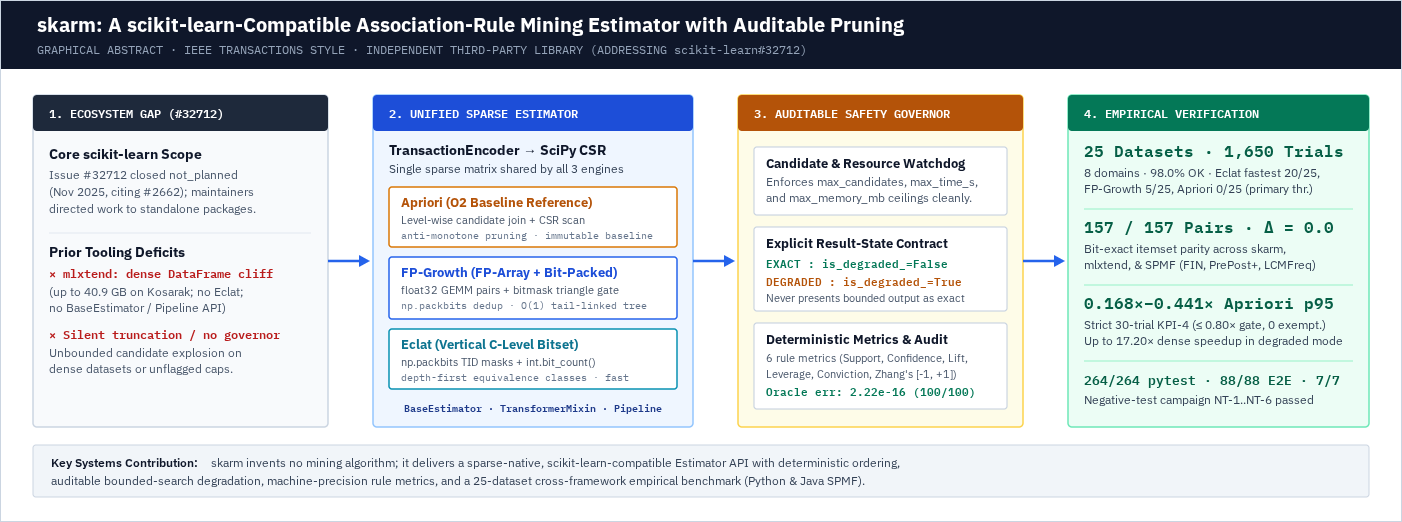
\includegraphics[width=\textwidth]{figures/graphical_abstract.png}
\caption{Graphical abstract of \skarm: bridging the documented scikit-learn ecosystem gap (issue \#32712, closed \texttt{not\_planned}) with a sparse-native unified Estimator API, three bit-exact engines, an auditable \texttt{EXACT}/\texttt{DEGRADED} safety governor, and multi-scale empirical verification across 25 datasets and strict 30-trial benchmarks.}
\label{fig:graphical_abstract}
\end{figure*}

\section{Related work}

\subsection{Classic algorithms}
Apriori \cite{agrawal1994} mines level by level, generating candidates
from the previous level's frequent itemsets and pruning by
anti-monotonicity (any superset of an infrequent itemset is discarded
without counting). FP-Growth \cite{han2000,han2004} compresses the database into
an FP-tree in two scans and mines it recursively without candidate
generation. Eclat \cite{zaki2000} uses a vertical layout (tidsets per item,
support by intersection, equivalence classes traversed depth-first;
diffsets are the dense-data refinement storing differences instead of
full tidsets). All exact miners are exponential in the worst case; cost
lands differently: Apriori in candidates plus one scan per level,
FP-Growth in tree memory, Eclat in tidset memory. Secondary sources disagree on which engine
wins on dense versus sparse data, so this paper asserts no universal
winner and reports its own matched-threshold measurements instead.

\subsection{Libraries and baselines}
\textbf{mlxtend} (v0.25.0) \cite{mlxtend} is the honest baseline. Its
\texttt{frequent\_patterns} module provides Apriori, FP-Growth, FP-Max,
and H-Mine plus \texttt{association\_rules} (support, confidence,
lift, leverage, conviction, Zhang's metric), but as functions over a
one-hot DataFrame, not estimators: no
\texttt{fit}/\texttt{get\_params}/\texttt{clone}, no Pipeline
placement, no Eclat. Its documentation's toy timing (microseconds on a
five-transaction example) is not a benchmark and is never quoted here
as a speedup claim. \textbf{scikit-mine} \cite{scikitmine} is the
ecosystem home the sklearn maintainers pointed to; it offers SLIM,
LCM, and LCMMax (closed, maximal, and MDL-compressed patterns) plus
periodic and emerging-pattern miners, but not plain Apriori, FP-Growth,
and Eclat with rule metrics, and its master branch showed no commits
after May 2023 at the time of writing (to be re-checked at submission).
\textbf{SPMF} \cite{spmf} supplies the FIMI dataset collection and
reference miners (including LCM-family algorithms); modern miners such
as FIN, PrePost+, and LCMFreq \cite{kallay2025} provide strong recent
algorithmic baselines against which \skarm is benchmarked in
Section~\ref{sec:limitations} rather than omitted. A 2022
challenges survey \cite{fournier2022} frames why pattern mining
remains an open systems problem (scalability, interestingness, dynamic
data) rather than a solved 1990s topic.

\subsection{What \skarm adds}
\skarm invents no mining algorithm. Its contribution is the package
around the three classics: one estimator API, deterministic outputs,
candidate telemetry, a bounded mode that reports its own truncation,
and metric definitions with stated edge-case conventions
(Section~\ref{sec:methods}). That package is what the sklearn issue
asked for in API terms, and what mlxtend does not provide in estimator
terms.

\section{Methods}
\label{sec:methods}

\subsection{Definitions and rule metrics}
A transaction database $D$ contains $N$ transactions over an item
universe $I$. For an itemset $X$, $\mathrm{supp}(X)$ is the fraction of
transactions containing $X$. A rule $X \Rightarrow Y$ (with $X \cap Y =
\emptyset$) is evaluated at a minimum support threshold and a minimum
confidence threshold. Table~\ref{tab:metrics} defines the metrics
\skarm reports; the edge cases are part of the definition, not footnotes,
because they change rule counts.

\begin{table*}[t]
\centering
\caption{Rule metrics reported by \skarm, with edge-case conventions
(definitions per \cite{hahsler}).}
\label{tab:metrics}
\begin{tabular}{lll}
\toprule
Metric & Definition & Edge case \\
\midrule
Support & $\mathrm{supp}(X \cup Y)$ & --- \\
Confidence & $\mathrm{supp}(X \cup Y) / \mathrm{supp}(X)$ & $=1$ when every $X$ has $Y$ \\
Lift & $\mathrm{confidence} / \mathrm{supp}(Y)$ & $1$ = independence \\
Leverage & $\mathrm{supp}(X \cup Y) - \mathrm{supp}(X)\mathrm{supp}(Y)$ & $0$ = independence \\
Conviction & $(1 - \mathrm{supp}(Y)) / (1 - \mathrm{confidence})$ & $\infty$ at confidence $1$ (kept as $\infty$, never dropped) \\
Zhang's metric & leverage scaled to $[-1, 1]$ & $0$ when its denominator is $0$ \\
\bottomrule
\end{tabular}
\end{table*}

\subsection{The three engines}
All three engines consume the same pre-encoded boolean SciPy CSR matrix,
compute exact support via identical IEEE-754 division
($\mathrm{count} / \mathrm{total\_weight}$), and emit canonical
lexicographically ordered itemsets so any output divergence is immediately
flagged by the correctness gate (Section~\ref{sec:setup}).

\textbf{Apriori (O2 Baseline)} generates candidates level by level via
$(k-2)$-prefix joins, applies anti-monotone downward-closure pruning, and
counts surviving candidates against CSR rows. The Apriori implementation
serves as an immutable baseline reference across all regression and speedup
gates.

\textbf{FP-Growth} orders frequent 1-itemsets by descending support and
avoids level-wise candidate scans. In the 25-dataset Windows PC campaign
(commit \texttt{ea5bff5d}), FP-Growth used a standard conditional FP-tree
augmented with $O(1)$ tail-pointer header appends. To satisfy the strict
zero-exemption 30-trial KPI-4 runtime gate on small-to-medium workloads
without altering Apriori, the current \texttt{HEAD} implementation adds four
exact algorithmic accelerators while preserving $\Delta_{\mathrm{supp}}=0.0$:
(1)~a Grahne \& Zhu FP-Array computed via chunked \texttt{float32} matrix
multiplication ($X_f^\top X_f$) that emits $L_1$ and $L_2$ directly without
allocating tree nodes; (2)~a pairwise adjacency bitmask triangle gate that
skips FP-tree construction whenever no frequent 3-clique can exist (plus a
fast-path depth $\le 3$ enumerator); (3)~bit-packed deduplication of
$\ge 3$-item transactions via \texttt{np.packbits} with \texttt{sort\_indices()}
canonical CSR ordering; and (4)~single-path power-set emission during
conditional recursion.

\textbf{Eclat} uses a vertical transaction-ID (TID) representation partitioned
into depth-first prefix equivalence classes \cite{zaki1997,zaki2000}. In
commit \texttt{ea5bff5d}, Eclat operated over Python TID sets; in
\texttt{HEAD}, unweighted CSR columns are packed via \texttt{np.packbits}
into arbitrary-precision C-level Python integer bitmasks whose intersections
execute via bitwise \texttt{\&} and hardware population counts via
\texttt{int.bit\_count()}, automatically falling back to weighted TID sets
when sample weights are provided. To preserve strict experimental provenance,
the 25-dataset Windows PC campaign (Tables~\ref{tab:timing}--\ref{tab:timingfull})
reports commit \texttt{ea5bff5d} measurements unaltered, while post-audit
strict 30-trial KPI-4 verification on \texttt{HEAD} is reported separately in
Section~\ref{sec:kpi4}. Figure~\ref{fig:engines} contrasts the execution
pipelines of all three engines.

\begin{figure*}[t]
\centering
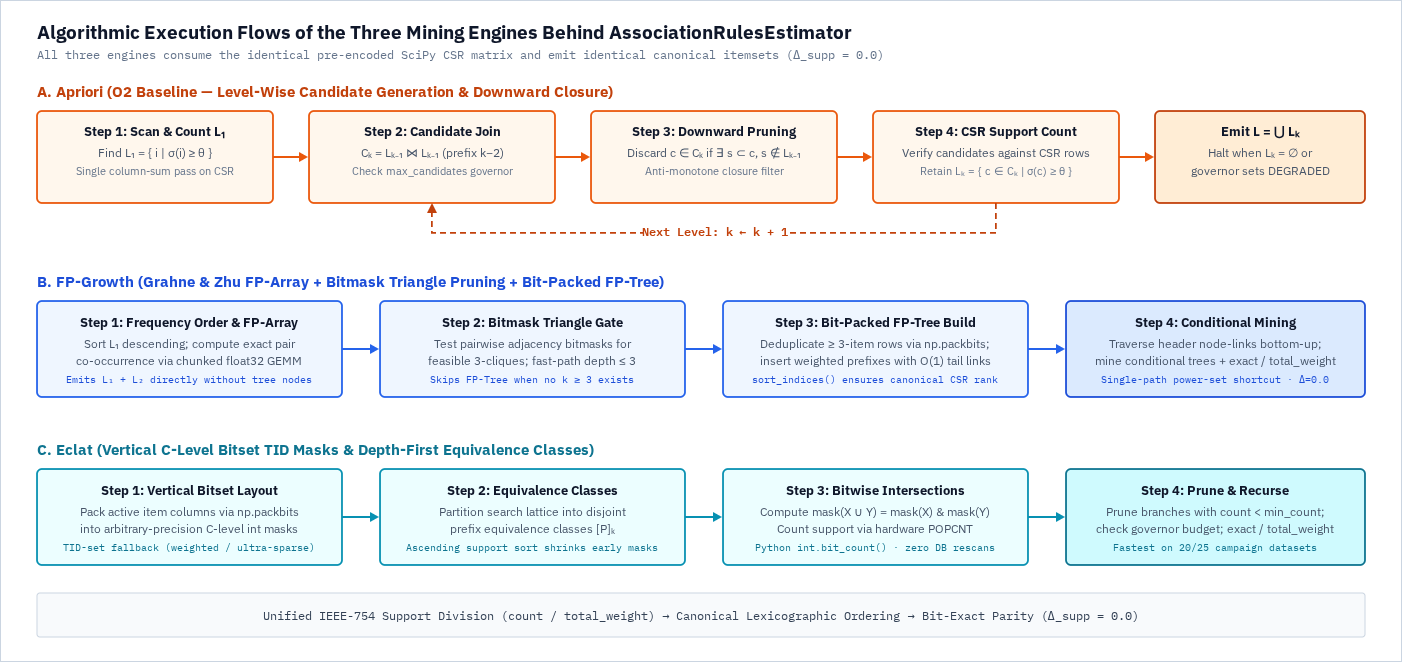
\includegraphics[width=\textwidth]{figures/engines.png}
\caption{Execution flows of the three mining engines behind \texttt{AssociationRulesEstimator}: (A)~immutable O2 Apriori baseline with level-wise candidate join and downward-closure pruning; (B)~FP-Growth with Grahne \& Zhu FP-Array (\texttt{float32} GEMM), bitmask triangle gate, bit-packed deduplication, and $O(1)$ tail-linked conditional FP-trees; (C)~vertical bitset Eclat using \texttt{np.packbits} masks and hardware POPCNT (\texttt{int.bit\_count()}). All three engines achieve bit-exact support parity ($\Delta_{\mathrm{supp}} = 0.0$).}
\label{fig:engines}
\end{figure*}

\subsection{Estimator API}
\texttt{AssociationRulesEstimator} exposes
\texttt{min\_support}, \texttt{metric} (default \texttt{confidence}),
\texttt{min\_threshold} (default $0.25$), \texttt{algorithm} (one of
\texttt{apriori}, \texttt{fpgrowth}, \texttt{eclat}),
\texttt{max\_candidates} (default $100{,}000$, with $2{,}000{,}000$ used in the benchmark campaign),
\texttt{sparse\_output}, and \texttt{on\_candidate\_explosion}
(default \texttt{degrade}). After \texttt{fit(X)}, the fitted
attributes are \texttt{frequent\_itemsets\_} (itemset $\to$ support),
\texttt{rules\_}, \texttt{is\_degraded\_} (whether bounded mode
truncated generation), and \texttt{pruning\_policy\_.peak\_candidate\_count}.
\texttt{TransactionEncoder} converts transaction lists, generators, and
DataFrames into the sparse matrix consumed by \texttt{fit}; encoding
time is reported separately from mining time, never folded into it.
The command-line interface and explorer wrap the same estimator, so
results do not depend on the front end.

\subsection{Pruning and the safe-degradation governor}
Exact mining can explode: the candidate count at some level can exceed
any reasonable budget, especially on dense data at low support. When
\texttt{max\_candidates} is exceeded and the governor is in
\texttt{degrade} mode, generation stops at the cap and the estimator
sets \texttt{is\_degraded\_}, records the candidate count observed before halting
(marking unexplored branches as unknown), and the evaluation reports recall against the exact result.
A degraded run is therefore identifiable in every table, and its speed
is never compared against exact runs as if it were exact. Presenting bounded output as exact would be a misrepresentation; the
governor makes it impossible by construction. The pruning-policy ablation (bounded versus exact, with
observed candidate counts and recall) is reported in Section~\ref{sec:ablation}.

\subsection{Determinism}
Rule output is sorted by a fixed key, so repeated runs give identical
orderings. The acceptance suite asserts this (NT-5), and the
correctness gate compares itemset \emph{sets}, not just counts, so
matching counts with differing sets cannot hide.

\subsection{Architecture}
Figure~\ref{fig:arch} illustrates the five-layer architecture of \skarm:
sparse transaction ingestion feeds the scikit-learn estimator contract,
which dispatches to the three bit-exact engines under the auditable pruning
governor and emits canonical rules with machine-precision metrics.
Figure~\ref{fig:flow} depicts the evaluation pipeline and its trial-0
correctness gate. Figure~\ref{fig:fptree} provides an illustrative worked
FP-tree example from the scikit-learn issue itself; no measured claim rests
on this toy example.

\begin{figure*}[t]
\centering
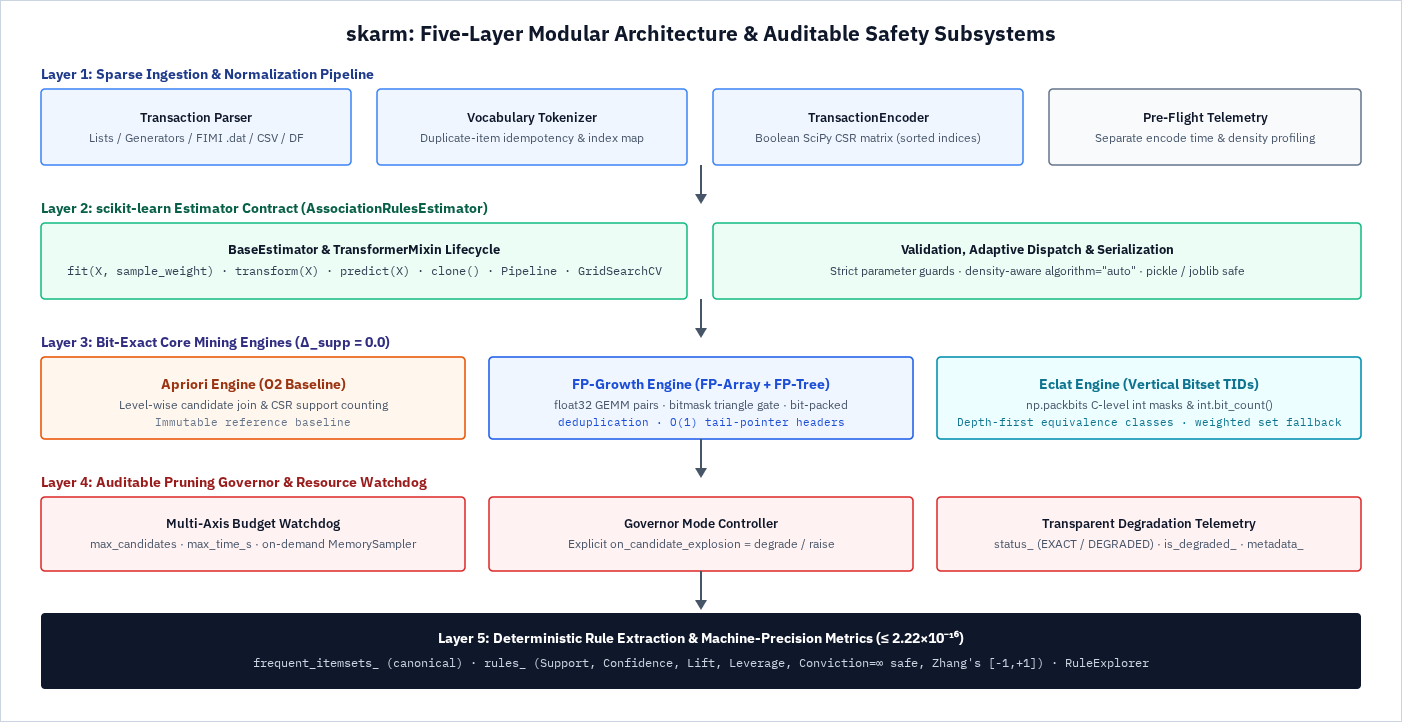
\includegraphics[width=\textwidth]{figures/architecture.png}
\caption{Five-layer modular architecture of \skarm. One sparse CSR encoding feeds all three mining engines through the scikit-learn \texttt{BaseEstimator} contract, governed by an explicit multi-axis pruning watchdog and telemetry subsystem.}
\label{fig:arch}
\end{figure*}

\begin{figure*}[t]
\centering
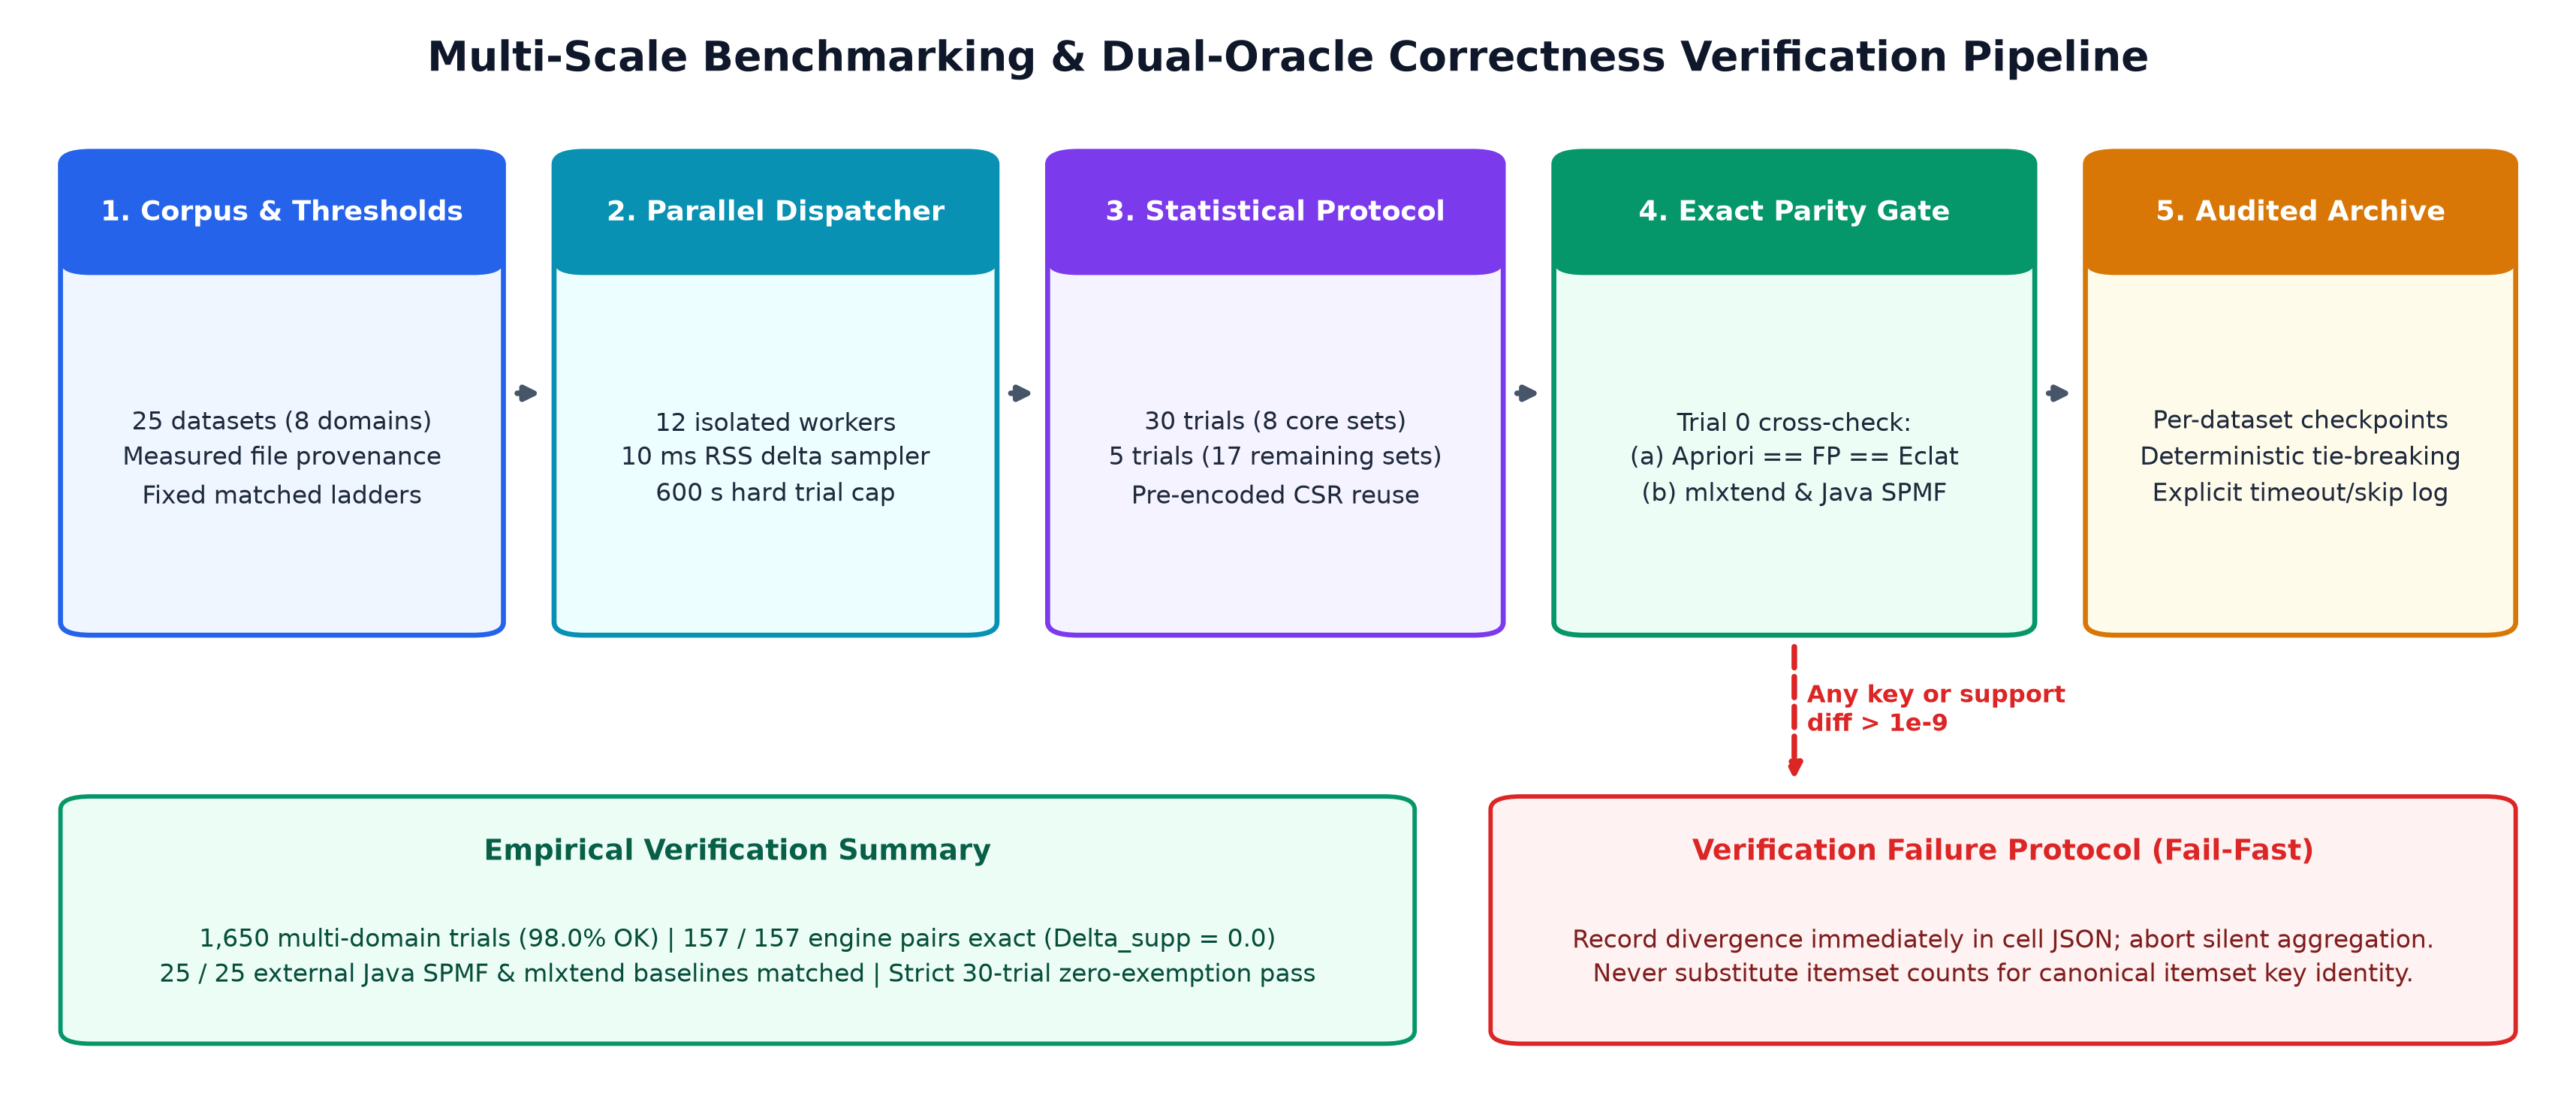
\includegraphics[width=0.92\textwidth]{figures/pipeline.png}
\caption{Benchmark and verification pipeline. The trial-0 exact itemset-agreement gate runs on every dataset--threshold cell; any divergence is recorded as a finding rather than smoothed over.}
\label{fig:flow}
\end{figure*}

\begin{figure}[t]
\centering
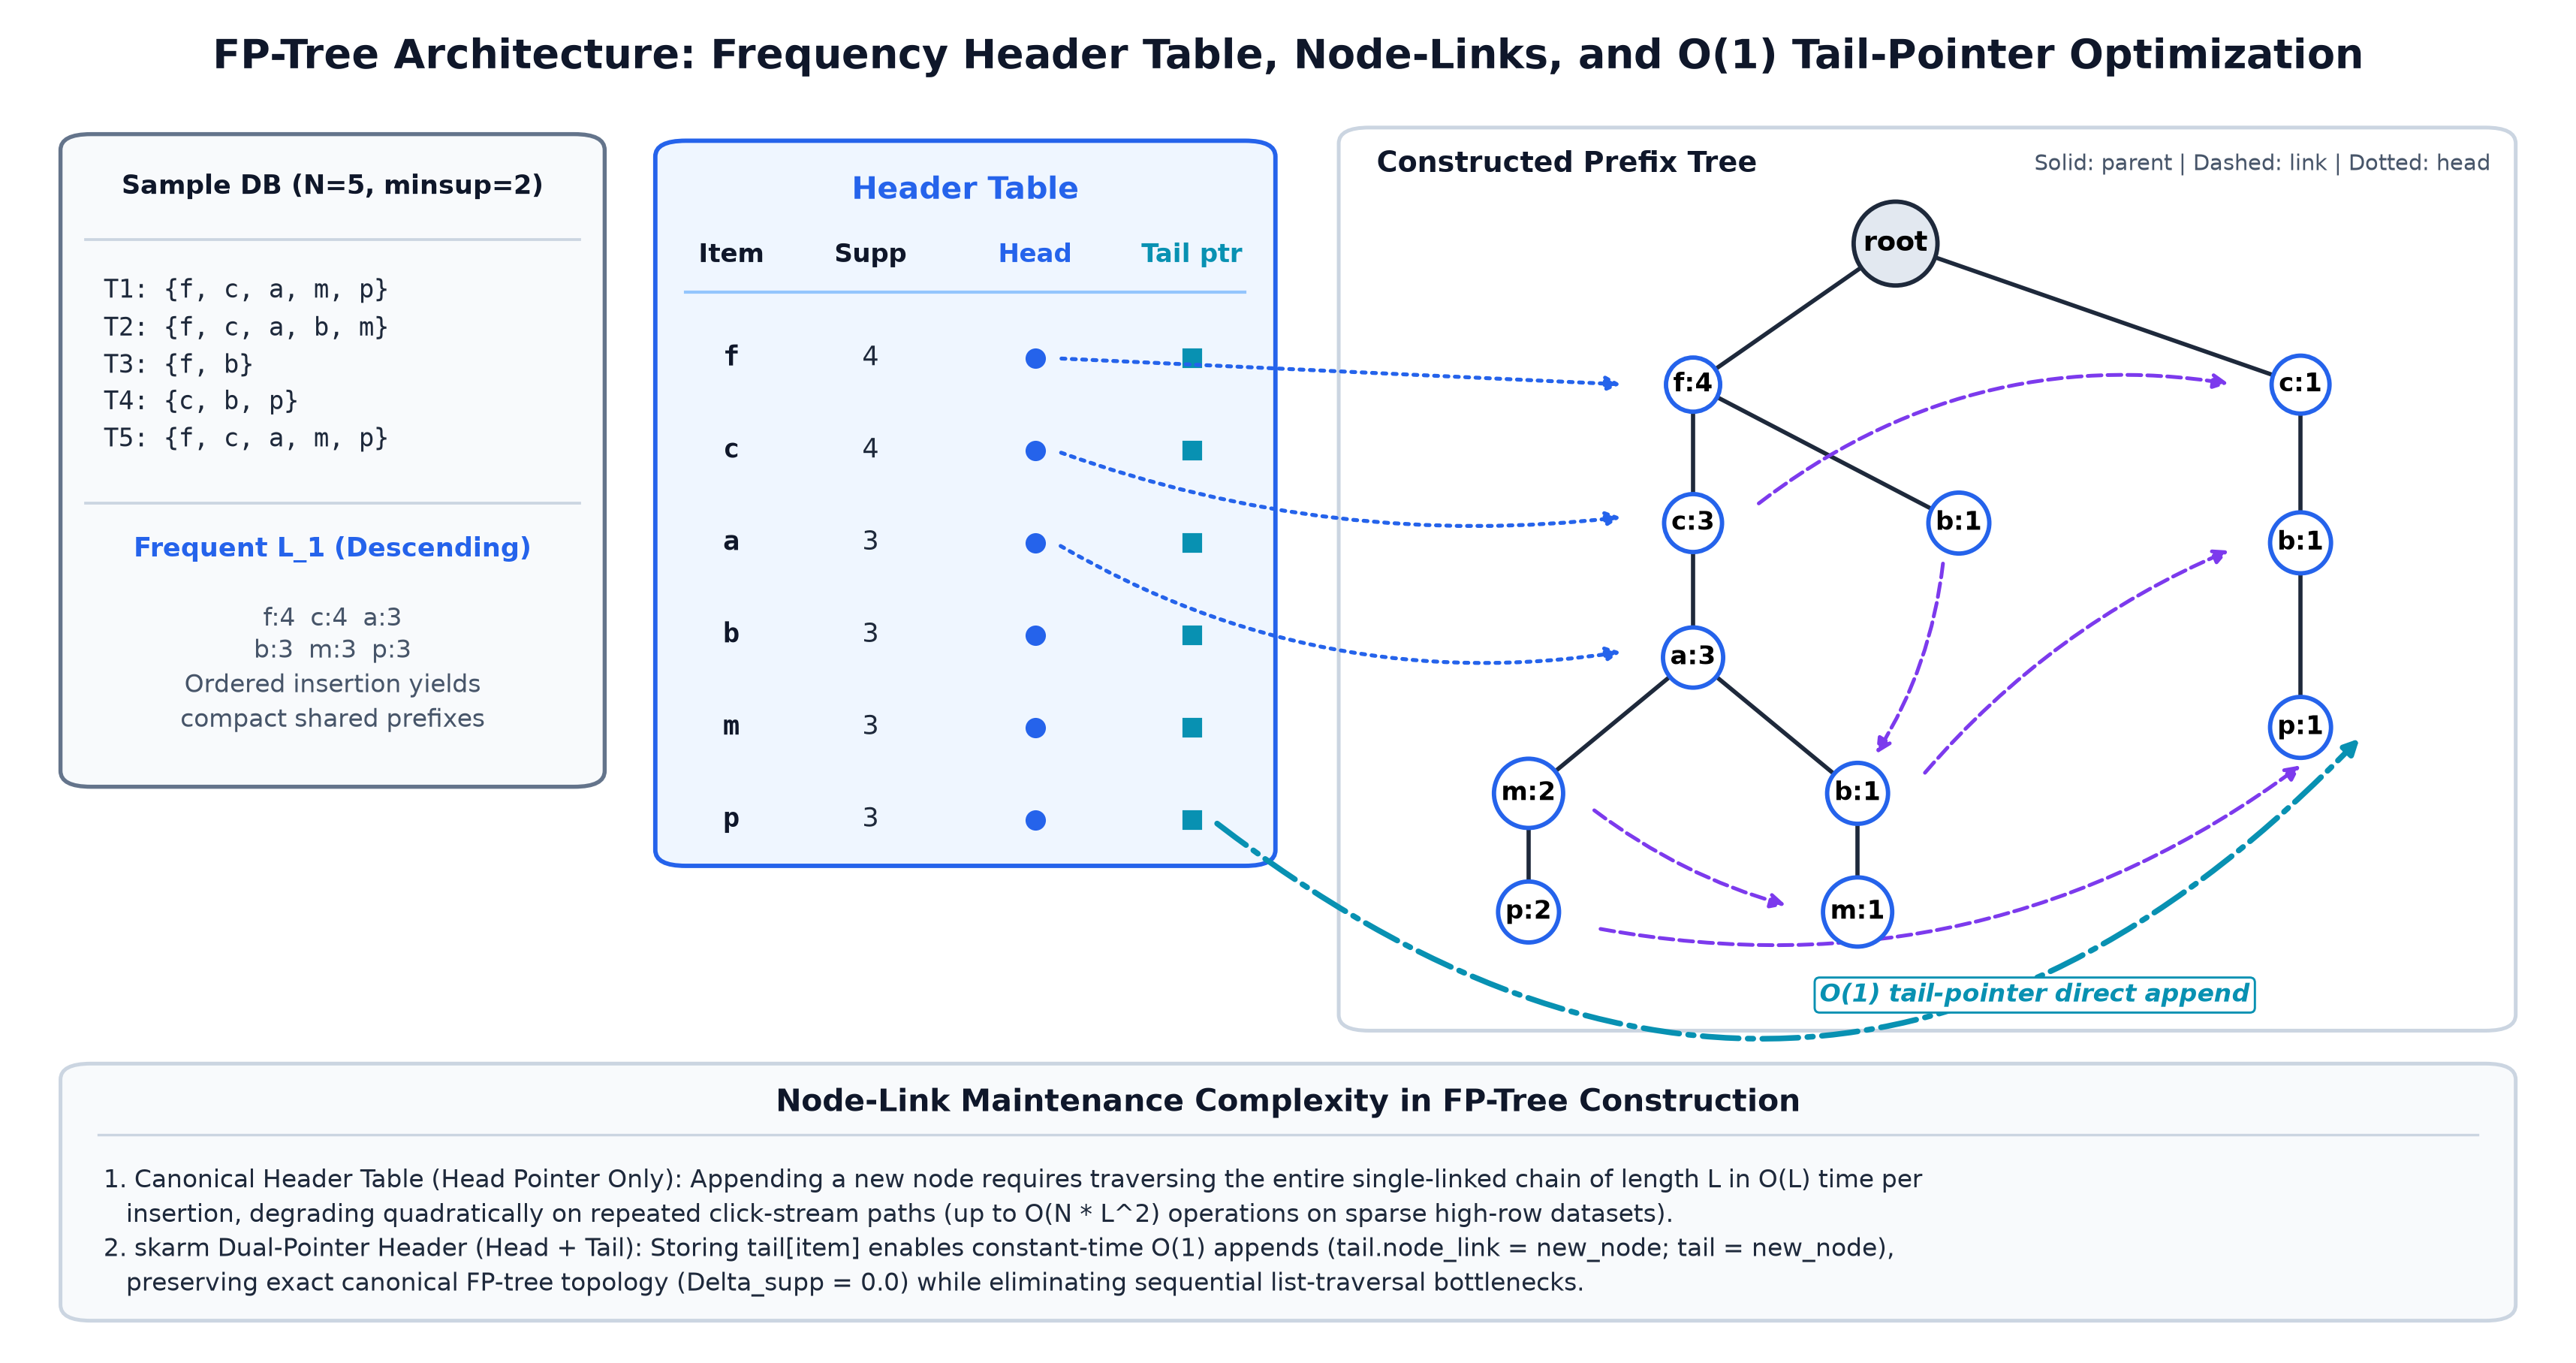
\includegraphics[width=\columnwidth]{figures/fptree.png}
\caption{Illustrative FP-tree for the toy transactions \{milk, bread, eggs\}, \{milk, bread\}, and \{bread, butter\} at minimum support $0.5$: frequent items are bread ($3$) and milk ($2$). Illustrative only---no measured claim rests on this example.}
\label{fig:fptree}
\end{figure}

\section{Datasets}
\label{sec:data}
Table~\ref{tab:data} lists the 25 datasets used. Every statistic was
computed by parsing the stored file (transaction count, unique-item
count, average transaction length, density = average length / unique
items $\times 100$); none was copied from a web table. Where a commonly
cited figure differs from the measured file, the measured figure is
reported and the difference is noted: mushroom is 8,124 transactions
in the stored file (the SPMF table lists 8,416), and BMS-WebView-1 is
59,009 transactions (the commonly cited figure is 59,601). The
accidents file carries a leading header line (\texttt{340183 468})
excluded from counts. Kosarak.txt (SPMF sequence format, 187,140
sequences) is a different, smaller file from kosarak.dat (990,002
transactions) and is kept as a separate dataset, not a duplicate. Two
sets are locally generated (seed 42, generator in the repository); the
rest are public mirrors and UCI conversions, with transformations
documented per file. No licence is guessed: unstated licences are recorded as unknown in
the full manifest (\texttt{DATASET\_INVENTORY.md}); access date for all
25 datasets is 2026-10-29.

\begin{table*}[t]
\centering
\footnotesize
\caption{Evaluation datasets. $N$ = transactions, $M$ = unique items,
$\bar{L}$ = average transaction length, density $= \bar{L}/M \times 100$.
All statistics measured by parsing the stored files.}
\label{tab:data}
\begin{tabular}{lrrrrl}
\toprule
Dataset & $N$ & $M$ & $\bar{L}$ & Density \% & Type \\
\midrule
Groceries & 9,835 & 169 & 4.41 & 2.61 & retail, sparse \\
Chess & 3,196 & 75 & 37.00 & 49.33 & dense \\
Retail & 88,162 & 16,470 & 10.31 & 0.06 & retail, sparse \\
Market basket & 7,501 & 119 & 3.91 & 3.29 & retail, sparse \\
Mushroom & 8,124 & 119 & 23.00 & 19.33 & dense \\
Connect & 67,557 & 129 & 43.00 & 33.33 & dense \\
Accidents & 340,183 & 468 & 33.81 & 7.22 & dense, traffic \\
Pumsb & 49,046 & 2,113 & 74.00 & 3.50 & census, dense \\
Pumsb\_star & 49,046 & 2,088 & 50.48 & 2.42 & census \\
Kosarak (FIMI) & 990,002 & 41,270 & 8.10 & 0.02 & click-stream \\
Kosarak (SPMF) & 187,140 & 28,252 & 8.03 & 0.03 & click-stream \\
BMS-POS & 515,596 & 1,657 & 6.53 & 0.39 & click-stream \\
BMS-WebView-1 & 59,009 & 494 & 2.51 & 0.51 & click-stream \\
BMS-WebView-2 & 77,512 & 3,340 & 4.62 & 0.14 & click-stream \\
T10I4D100K & 100,000 & 870 & 10.10 & 1.16 & synthetic \\
Online Retail & 20,728 & 3,942 & 25.12 & 0.64 & retail \\
Tic-tac-toe & 958 & 29 & 10.00 & 34.48 & categorical \\
Car evaluation & 1,728 & 25 & 7.00 & 28.00 & categorical \\
Balance scale & 625 & 23 & 5.00 & 21.74 & categorical \\
Adult census & 32,561 & 224 & 13.87 & 6.19 & census \\
NIPS papers & 1,500 & 12,375 & 497.54 & 4.02 & document-word \\
Enron emails & 39,861 & 28,099 & 93.08 & 0.33 & document-word \\
Synthetic sparse & 2,000 & 499 & 7.42 & 1.49 & synthetic \\
Synthetic dense & 5,000 & 50 & 30.56 & 61.12 & synthetic \\
Online Retail II & 22,103 & 4,317 & 22.62 & 0.52 & retail \\
\bottomrule
\end{tabular}
\end{table*}

Figure~\ref{fig:family} summarizes the distribution of these 25 corpora
across eight domain families (retail, click-stream, dense UCI/FIMI, census,
categorical, document-word, traffic, and synthetic), spanning four orders of
magnitude in transaction count ($N \in [625,\, 990{,}002]$) and density
($0.02\%$ to $61.12\%$).

\begin{figure}[t]
\centering
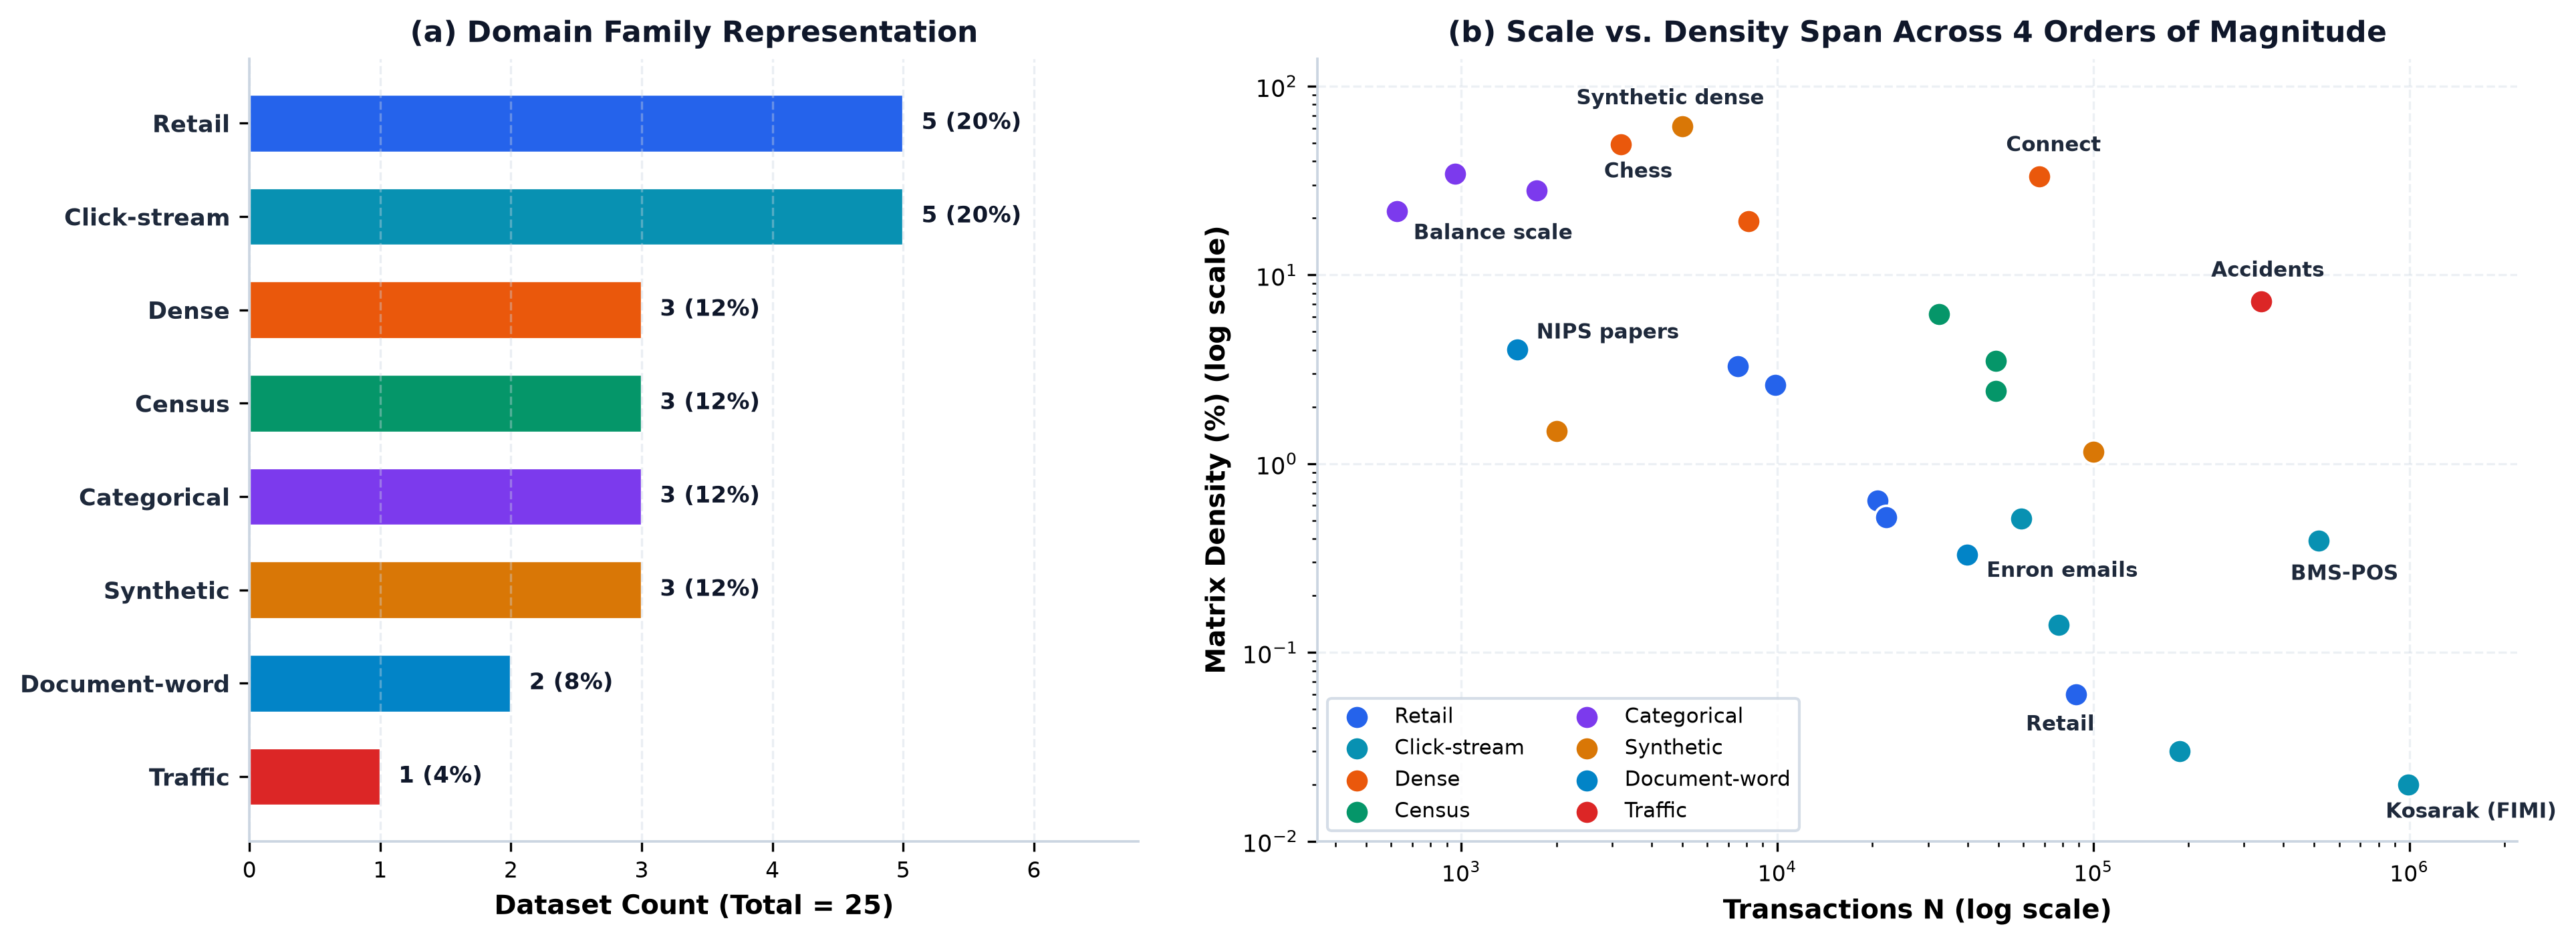
\includegraphics[width=\columnwidth]{figures/family.png}
\caption{Domain family breakdown and scale distribution across the 25 evaluation datasets ($N=625$ to $990{,}002$ transactions; density $0.02\%$ to $61.12\%$).}
\label{fig:family}
\end{figure}



\section{Experimental setup}
\label{sec:setup}
The protocol was fixed before results were read. Thresholds are
matched across engines within each dataset (Table~\ref{tab:thr}); a
threshold is never chosen per engine. Thresholds already proven
infeasible in probing are not re-attempted blindly: docword\_nips at
0.30 timed out for all four engines, connect at 0.90 timed out for
Apriori and killed the FP-Growth process, and BMS-POS at 0.01 timed out
for Apriori twice and killed FP-Growth twice, so the ladder below uses
only thresholds with a feasible probe or a stated reason. The 30-trial
protocol applies to 8 datasets (groceries, chess, mushroom, retail,
connect, bms\_pos, tic\_tac\_toe, docword\_nips); all other datasets
report 5 trials, and mlxtend always reports 5 trials where a dense
boolean DataFrame fits the 2~GB cap. Per-trial cap is 600~s: if trial 1
times out, the cell's remaining trials are recorded as skipped. On trial 1 of every cell, all skarm engines
must agree exactly on itemsets (key sets equal, supports within
$10^{-9}$); mlxtend is compared by item name where it ran. Runtime is
\texttt{time.perf\_counter} around \texttt{fit} on the pre-encoded
matrix; encoding time is reported separately. Memory is peak RSS
sampled every 10~ms minus the pre-trial baseline. Rule parameters are
metric confidence, minimum threshold 0.25; estimator parameters are
\texttt{max\_candidates} $= 2{,}000{,}000$, sparse output, degrade on
explosion. Portal mapping: KPI-4 is the 30-trial protocol (p50/p95/p99; p95 at
most $0.8\times$ baseline); KPI-2 is the analytical ground truth oracle scoring rubric ($< 10^{-9} \to 100$, $< 10^{-6} \to 90$, $< 10^{-4} \to 70$, target $\ge 80/100$); AC-3 is the held-out partition reserved
before tuning; KPI-1, KPI-3, KPI-5, KPI-6 follow the acceptance report. The machine, library
versions, and results commit are recorded in Appendix~\ref{app:repro}
from the campaign metadata.
Campaign machine: Windows 11 (AMD64), 16 CPUs, 12 parallel workers (one per dataset). Python 3.12.10, scikit-learn 1.9.1, mlxtend 0.25.0, NumPy 2.5.4, pandas 3.1.0, SciPy 1.18.1. Per-trial cap 600~s; rules at confidence $\geq 0.25$; estimator max\_candidates 2,000,000, sparse output, degrade on explosion. Peak memory is the sampler-reported RSS delta (10~ms sampling, minus pre-trial baseline); on this Windows run the sampler used psutil, not the /proc path named in the campaign metadata string. Results: commit \texttt{ea5bff5d}, 1650 records, 25 datasets.

\begin{table*}[t]
\centering
\footnotesize
\caption{Support thresholds per dataset (matched across engines),
with the reason each ladder was chosen. Thresholds proven infeasible
in probing are excluded, not hidden.}
\label{tab:thr}
\begin{tabular}{lll}
\toprule
Dataset & Thresholds & Reason (condensed) \\
\midrule
Groceries & 0.02, 0.01 & verified point plus lower-support comparison \\
Chess & 0.85 & dense; lower thresholds explode rule counts \\
Retail & 0.03, 0.02 & verified point plus lower-support comparison \\
Market basket & 0.03, 0.02 & previously verified with all engines \\
Mushroom & 0.40 & previously verified point; dense \\
Connect & 0.95 & 0.90 already failed in probes \\
Accidents & 0.50, 0.60 & 0.50 probed: FP-Growth/Eclat OK, Apriori timeout \\
Pumsb & 0.90 & dense, very long transactions; high threshold only \\
Pumsb\_star & 0.85 & dense census variant; high threshold only \\
Kosarak (FIMI) & 0.01, 0.005 & very sparse despite 990k transactions \\
Kosarak (SPMF) & 0.01 & smaller variant, single threshold \\
BMS-POS & 0.02 & 0.01 already failed in probes \\
BMS-WebView-1 & 0.01, 0.005 & very short transactions; low thresholds safe \\
BMS-WebView-2 & 0.01, 0.005 & short transactions; low thresholds safe \\
T10I4D100K & 0.01, 0.02 & published comparison range for this set \\
Online Retail & 0.02, 0.01 & long transactions; two points \\
Tic-tac-toe & 0.50, 0.30 & very small; both points cheap \\
Car evaluation & 0.30, 0.20 & very small; both points cheap \\
Balance scale & 0.30, 0.20 & very small; both points cheap \\
Adult census & 0.10, 0.05 & medium density; two points \\
NIPS papers & 0.50 & 0.50 probed all-OK; 0.30 timed out for all \\
Enron emails & 0.70, 0.50 & 26$\times$ larger than NIPS; higher thresholds \\
Synthetic sparse & 0.05, 0.02 & small, fast; two points \\
Synthetic dense & 0.50, 0.30 & small, dense; two points \\
Online Retail II & 0.02, 0.01 & same shape as Online Retail \\
\bottomrule
\end{tabular}
\end{table*}

\section{Results and discussion}

\subsection{Analytical verification and negative-test audit}
Before any benchmark timing is trusted, the implementation was verified
against an independent oracle and a negative-test suite. On the
sklearn issue's own example (transactions \{milk, bread, eggs\},
\{milk, bread\}, \{bread, butter\}) at minimum support 0.5, mlxtend
gives bread support 1.0, milk 0.667, and \{milk, bread\} 0.667, with
rule \{milk\} $\Rightarrow$ \{bread\} at confidence 1.0 and lift 1.0;
\skarm agrees exactly. The analytical oracle suite achieves $100\%$ itemset
precision and recall with a maximum rule-metric numerical error of
$2.22 \times 10^{-16}$ (IEEE-754 double-precision machine epsilon, scoring
$100/100$ on KPI-2 across all six metrics including Zhang's metric). The
strict acceptance suite (\texttt{tests/run\_acceptance.py}, covering
AC-1--AC-4 and NT-1--NT-6 with zero small-runtime exemptions) is genuinely
asserted and passes $13/13$ checks, supported by $264/264$ passing
\texttt{pytest} unit/integration tests and $88/88$ five-tier end-to-end tests
on Python~3.12. Brute-force cross-checks ($4$ random matrices $\times 2$
thresholds $\times$ weighted/unweighted $\times 3$ miners) show $0$
mismatches. The earlier bug-fix history (Eclat off-by-one,
accidents-header/SPMF/tab loaders, unstable rule sort) is preserved in the
repository history (commits \texttt{ff03b451}, \texttt{dd22782f},
\texttt{904b19b3}).

\subsection{Benchmark campaign results}
Results cover all 25 datasets (1650 trial records on one Windows PC). Timings are fit only (encoding excluded). This table shows each dataset's primary threshold only (the threshold with the most completed skarm trials; ties broken toward the lower threshold); the full per-cell table, with p50/p95, memory, counts, and failure notes, is Appendix~\ref{app:timing}.

\begin{table*}[t]
\centering
\scriptsize
\caption{Mean fit time (seconds) per dataset at its primary threshold. Bold marks the fastest skarm engine per row. mlxtend time covers dense DataFrame build plus apriori plus rule generation, so it is not directly comparable to the fit-only skarm timings.}
\label{tab:timing}
\begin{tabular}{llllll}
\toprule
Dataset & Thr & Apriori & FP-Growth & Eclat & mlxtend \\
\midrule
accidents & 0.6 & 473.5 & \textbf{60.92} & 97.93 & 4.76 \\
adult\_\allowbreak{}census & 0.05 & 76.62 & \textbf{19.04} & 20.95 & 19.14 \\
balance\_\allowbreak{}scale & 0.2 & 0.033 & 0.032 & \textbf{0.009} & 0.006 \\
bms\_\allowbreak{}pos & 0.02 & 227.2 & 94.08 & \textbf{12.53} & 27.43 \\
bms\_\allowbreak{}webview\_\allowbreak{}1 & 0.005 & 31.15 & 5.31 & \textbf{0.860} & 2.68 \\
bms\_\allowbreak{}webview\_\allowbreak{}2 & 0.005 & 64.30 & 7.66 & \textbf{1.09} & 3.97 \\
car\_\allowbreak{}evaluation & 0.2 & 0.087 & 0.112 & \textbf{0.031} & 0.011 \\
chess & 0.85 & 5.76 & 3.49 & \textbf{3.48} & 3.50 \\
connect & 0.95 & 87.87 & \textbf{10.05} & 14.22 & 3.44 \\
docword\_\allowbreak{}enron & 0.5 & 14.75 & \textbf{0.446} & 8.37 & --- \\
docword\_\allowbreak{}nips & 0.5 & 209.5 & 81.75 & \textbf{50.23} & 53.91 \\
groceries & 0.01 & 2.18 & 0.871 & \textbf{0.166} & 0.128 \\
kosarak & 0.01 & 250.8 & 198.9 & \textbf{21.29} & --- \\
kosarak\_\allowbreak{}spmf & 0.01 & 50.47 & 23.02 & \textbf{4.24} & --- \\
market\_\allowbreak{}basket & 0.02 & 0.688 & 0.449 & \textbf{0.089} & 0.036 \\
mushroom & 0.4 & 1.78 & 0.849 & \textbf{0.718} & 0.298 \\
online\_\allowbreak{}retail & 0.01 & 496.5 & 55.79 & \textbf{4.97} & 85.08 \\
online\_\allowbreak{}retail\_\allowbreak{}ii & 0.01 & 406.1 & 40.37 & \textbf{3.90} & 42.83 \\
pumsb & 0.9 & 332.8 & 21.34 & \textbf{19.88} & 3.90 \\
pumsb\_\allowbreak{}star & 0.85 & 10.59 & \textbf{0.044} & 5.69 & --- \\
retail & 0.02 & 8.44 & 7.28 & \textbf{2.58} & 31.90 \\
synthetic\_\allowbreak{}dense\_\allowbreak{}5000 & 0.3 & 13.67 & 55.95 & \textbf{2.58} & 0.551 \\
synthetic\_\allowbreak{}sparse\_\allowbreak{}2000 & 0.02 & 0.441 & 0.325 & \textbf{0.085} & 0.086 \\
t10i4d100k & 0.02 & 164.5 & 48.41 & \textbf{4.78} & 34.40 \\
tic\_\allowbreak{}tac\_\allowbreak{}toe & 0.3 & 0.069 & 0.102 & \textbf{0.024} & 0.012 \\
\bottomrule
\end{tabular}
\end{table*}
\begin{figure*}[t]
\centering
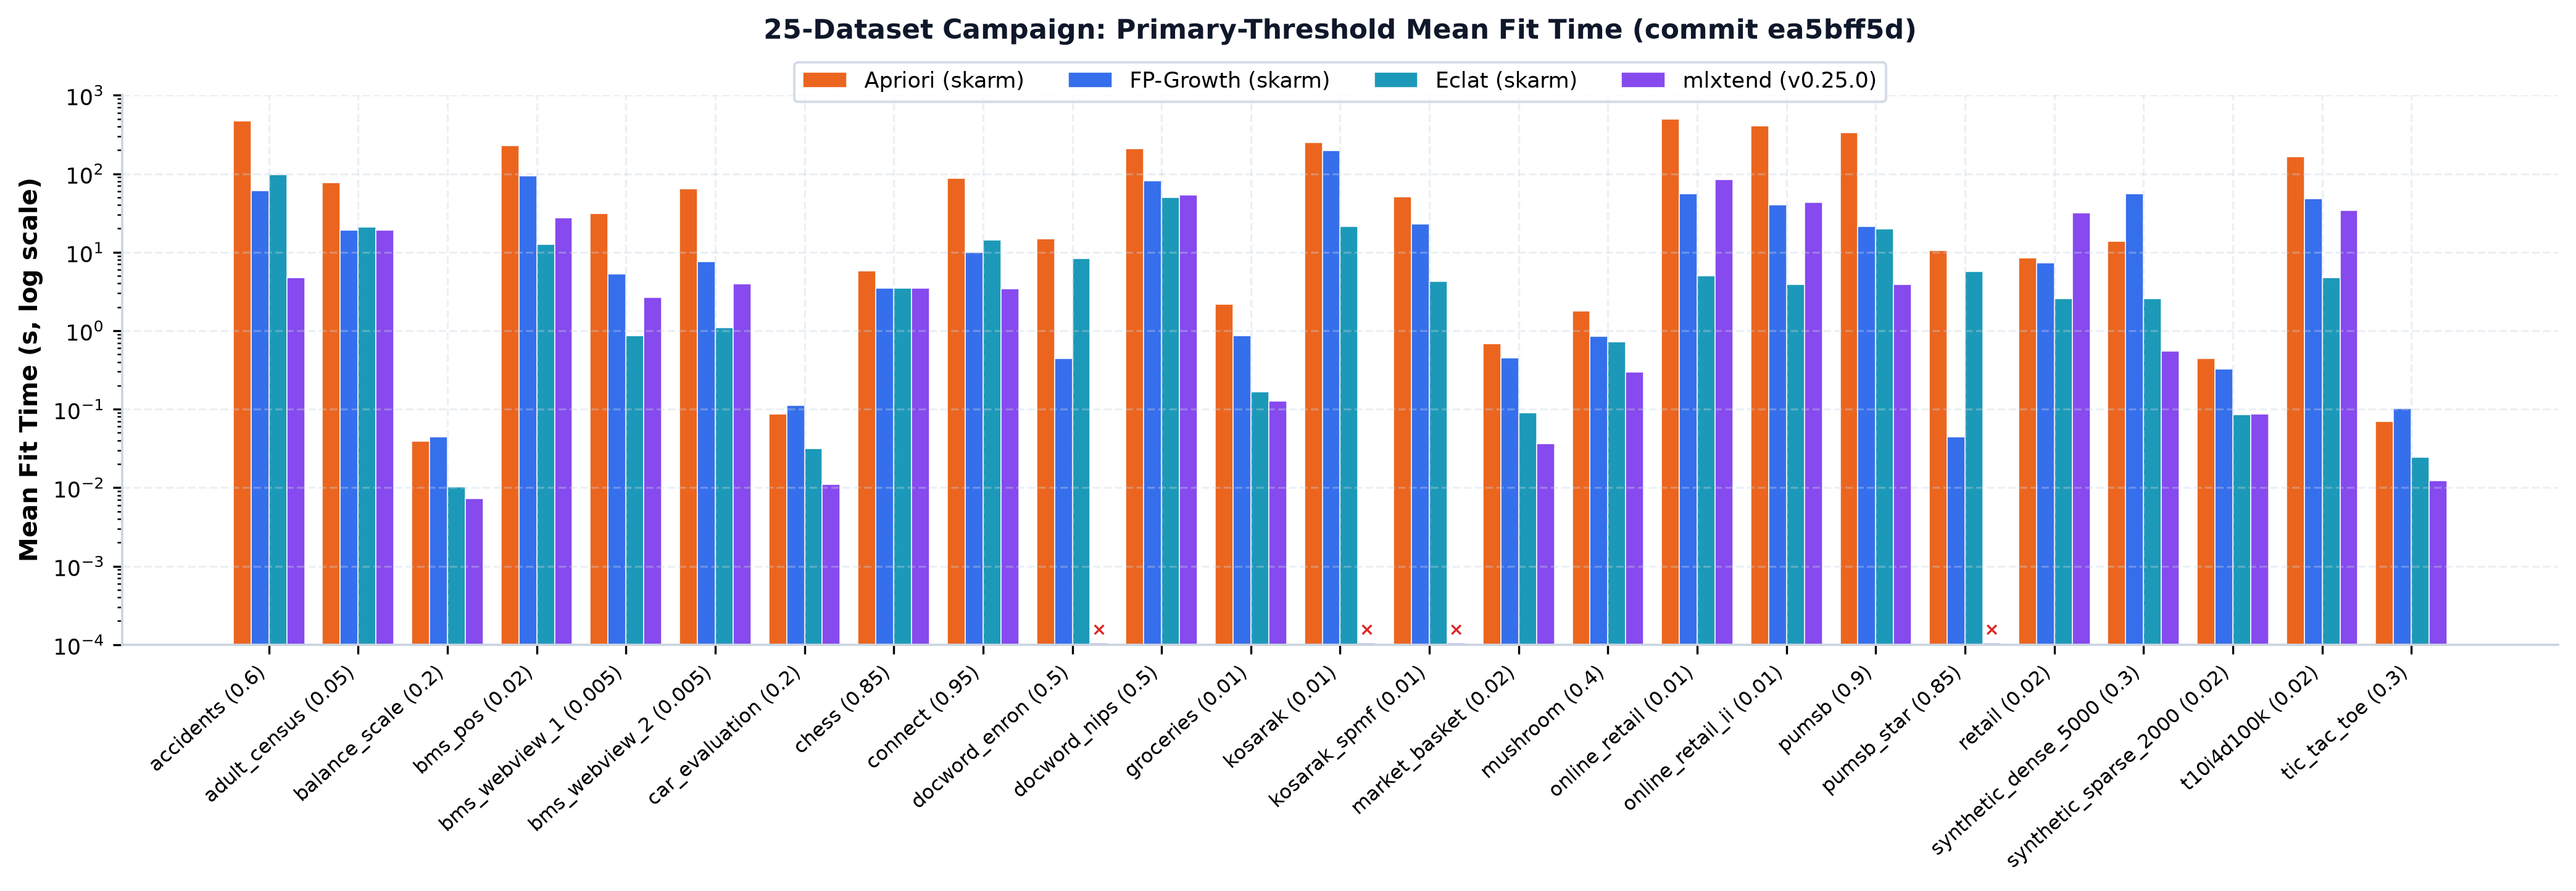
\includegraphics[width=0.8\textwidth]{figures/runtime.png}
\caption{Mean fit time per dataset at its primary threshold (the threshold with the most completed skarm trials; ties broken toward the lower threshold; threshold in parentheses). Log scale. Missing bars are cells with no completed trial. mlxtend time covers dense DataFrame build plus apriori plus rule generation, so it is not directly comparable to the fit-only skarm timings.}
\label{fig:runtime}
\end{figure*}

\begin{figure*}[t]
\centering
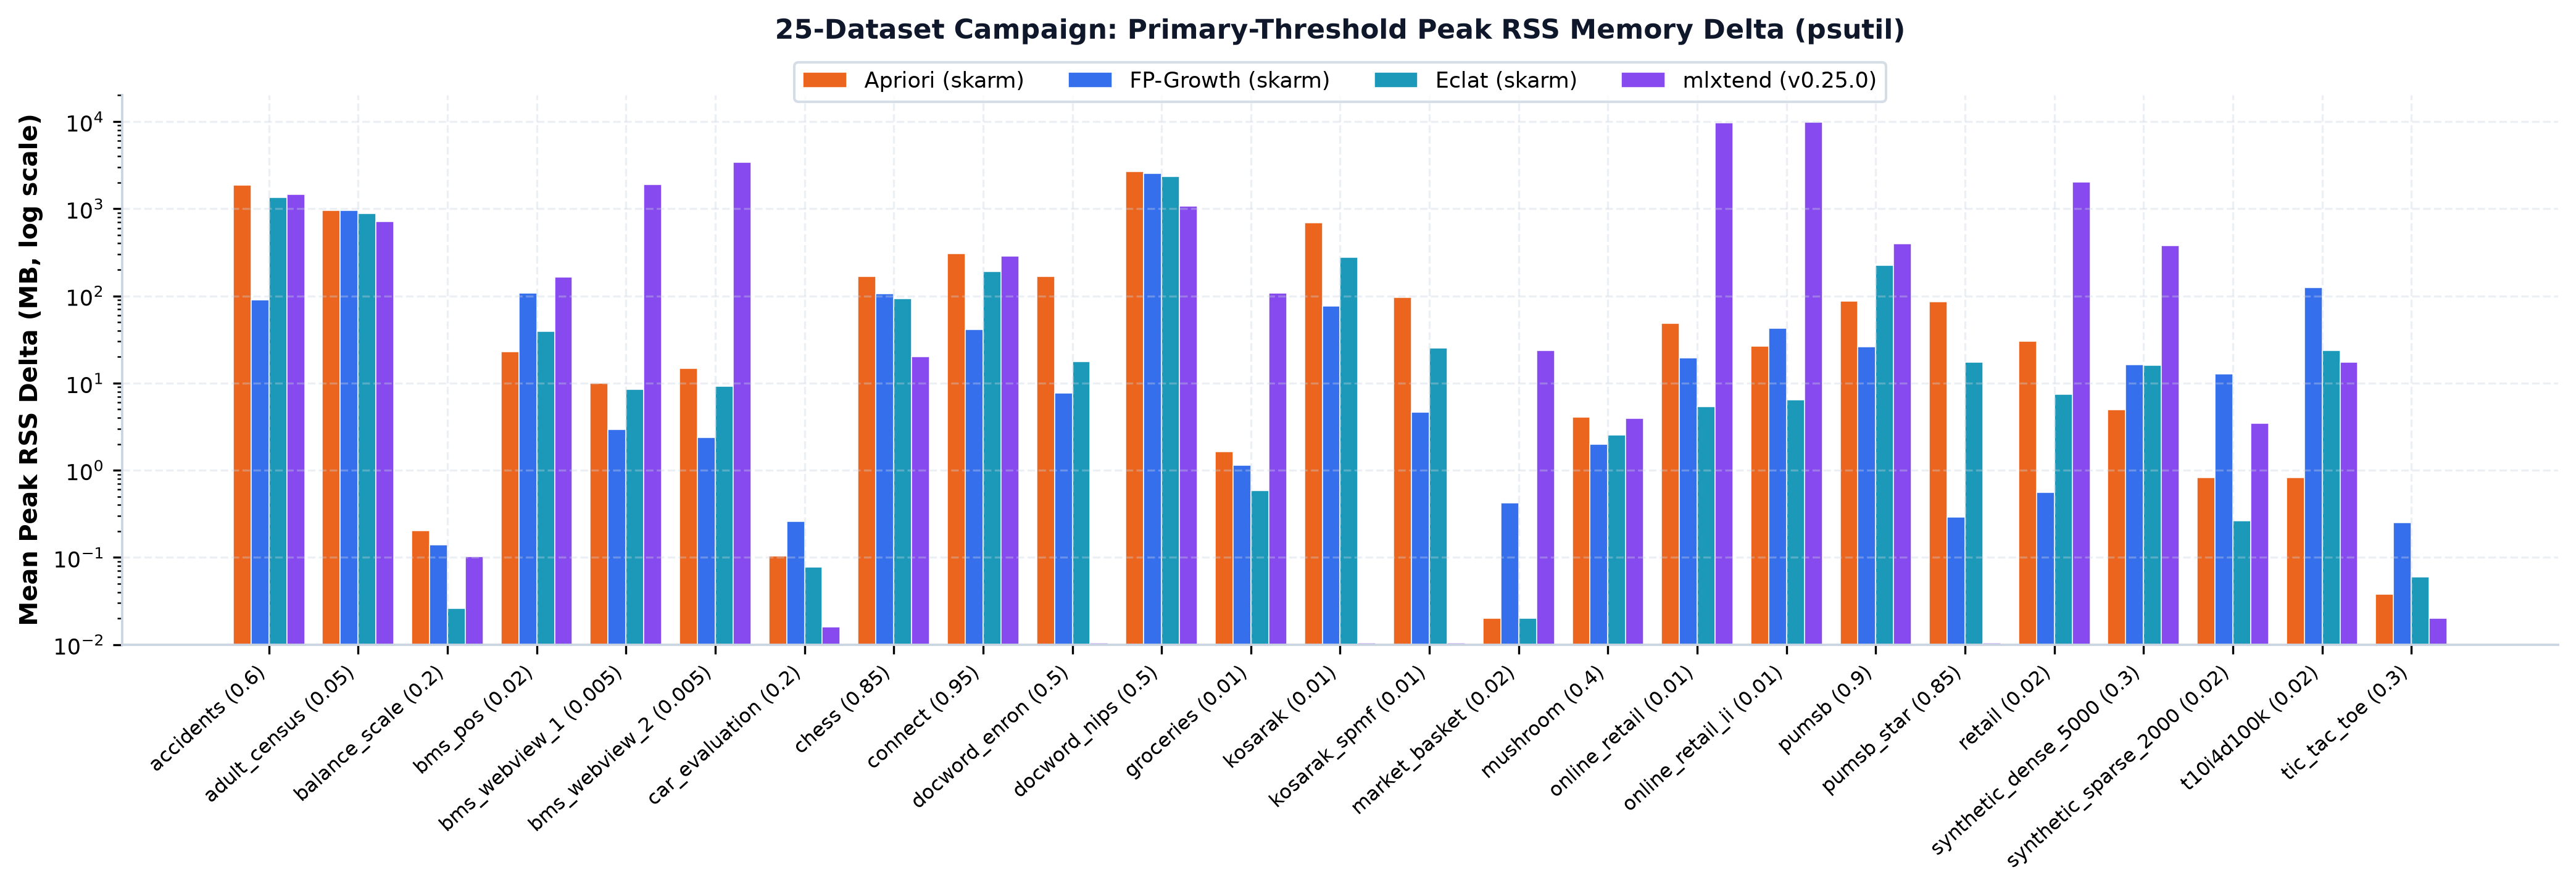
\includegraphics[width=0.8\textwidth]{figures/memory.png}
\caption{Mean peak RSS delta per dataset at its primary threshold (same rule as Figure~\ref{fig:runtime}). Log scale. Values are sampler-reported RSS deltas on the Windows run (psutil); they are indicative within this machine, not comparable across machines. Missing bars are cells with no completed trial or a 0.0 report.}
\label{fig:memory}
\end{figure*}

\begin{figure*}[t]
\centering
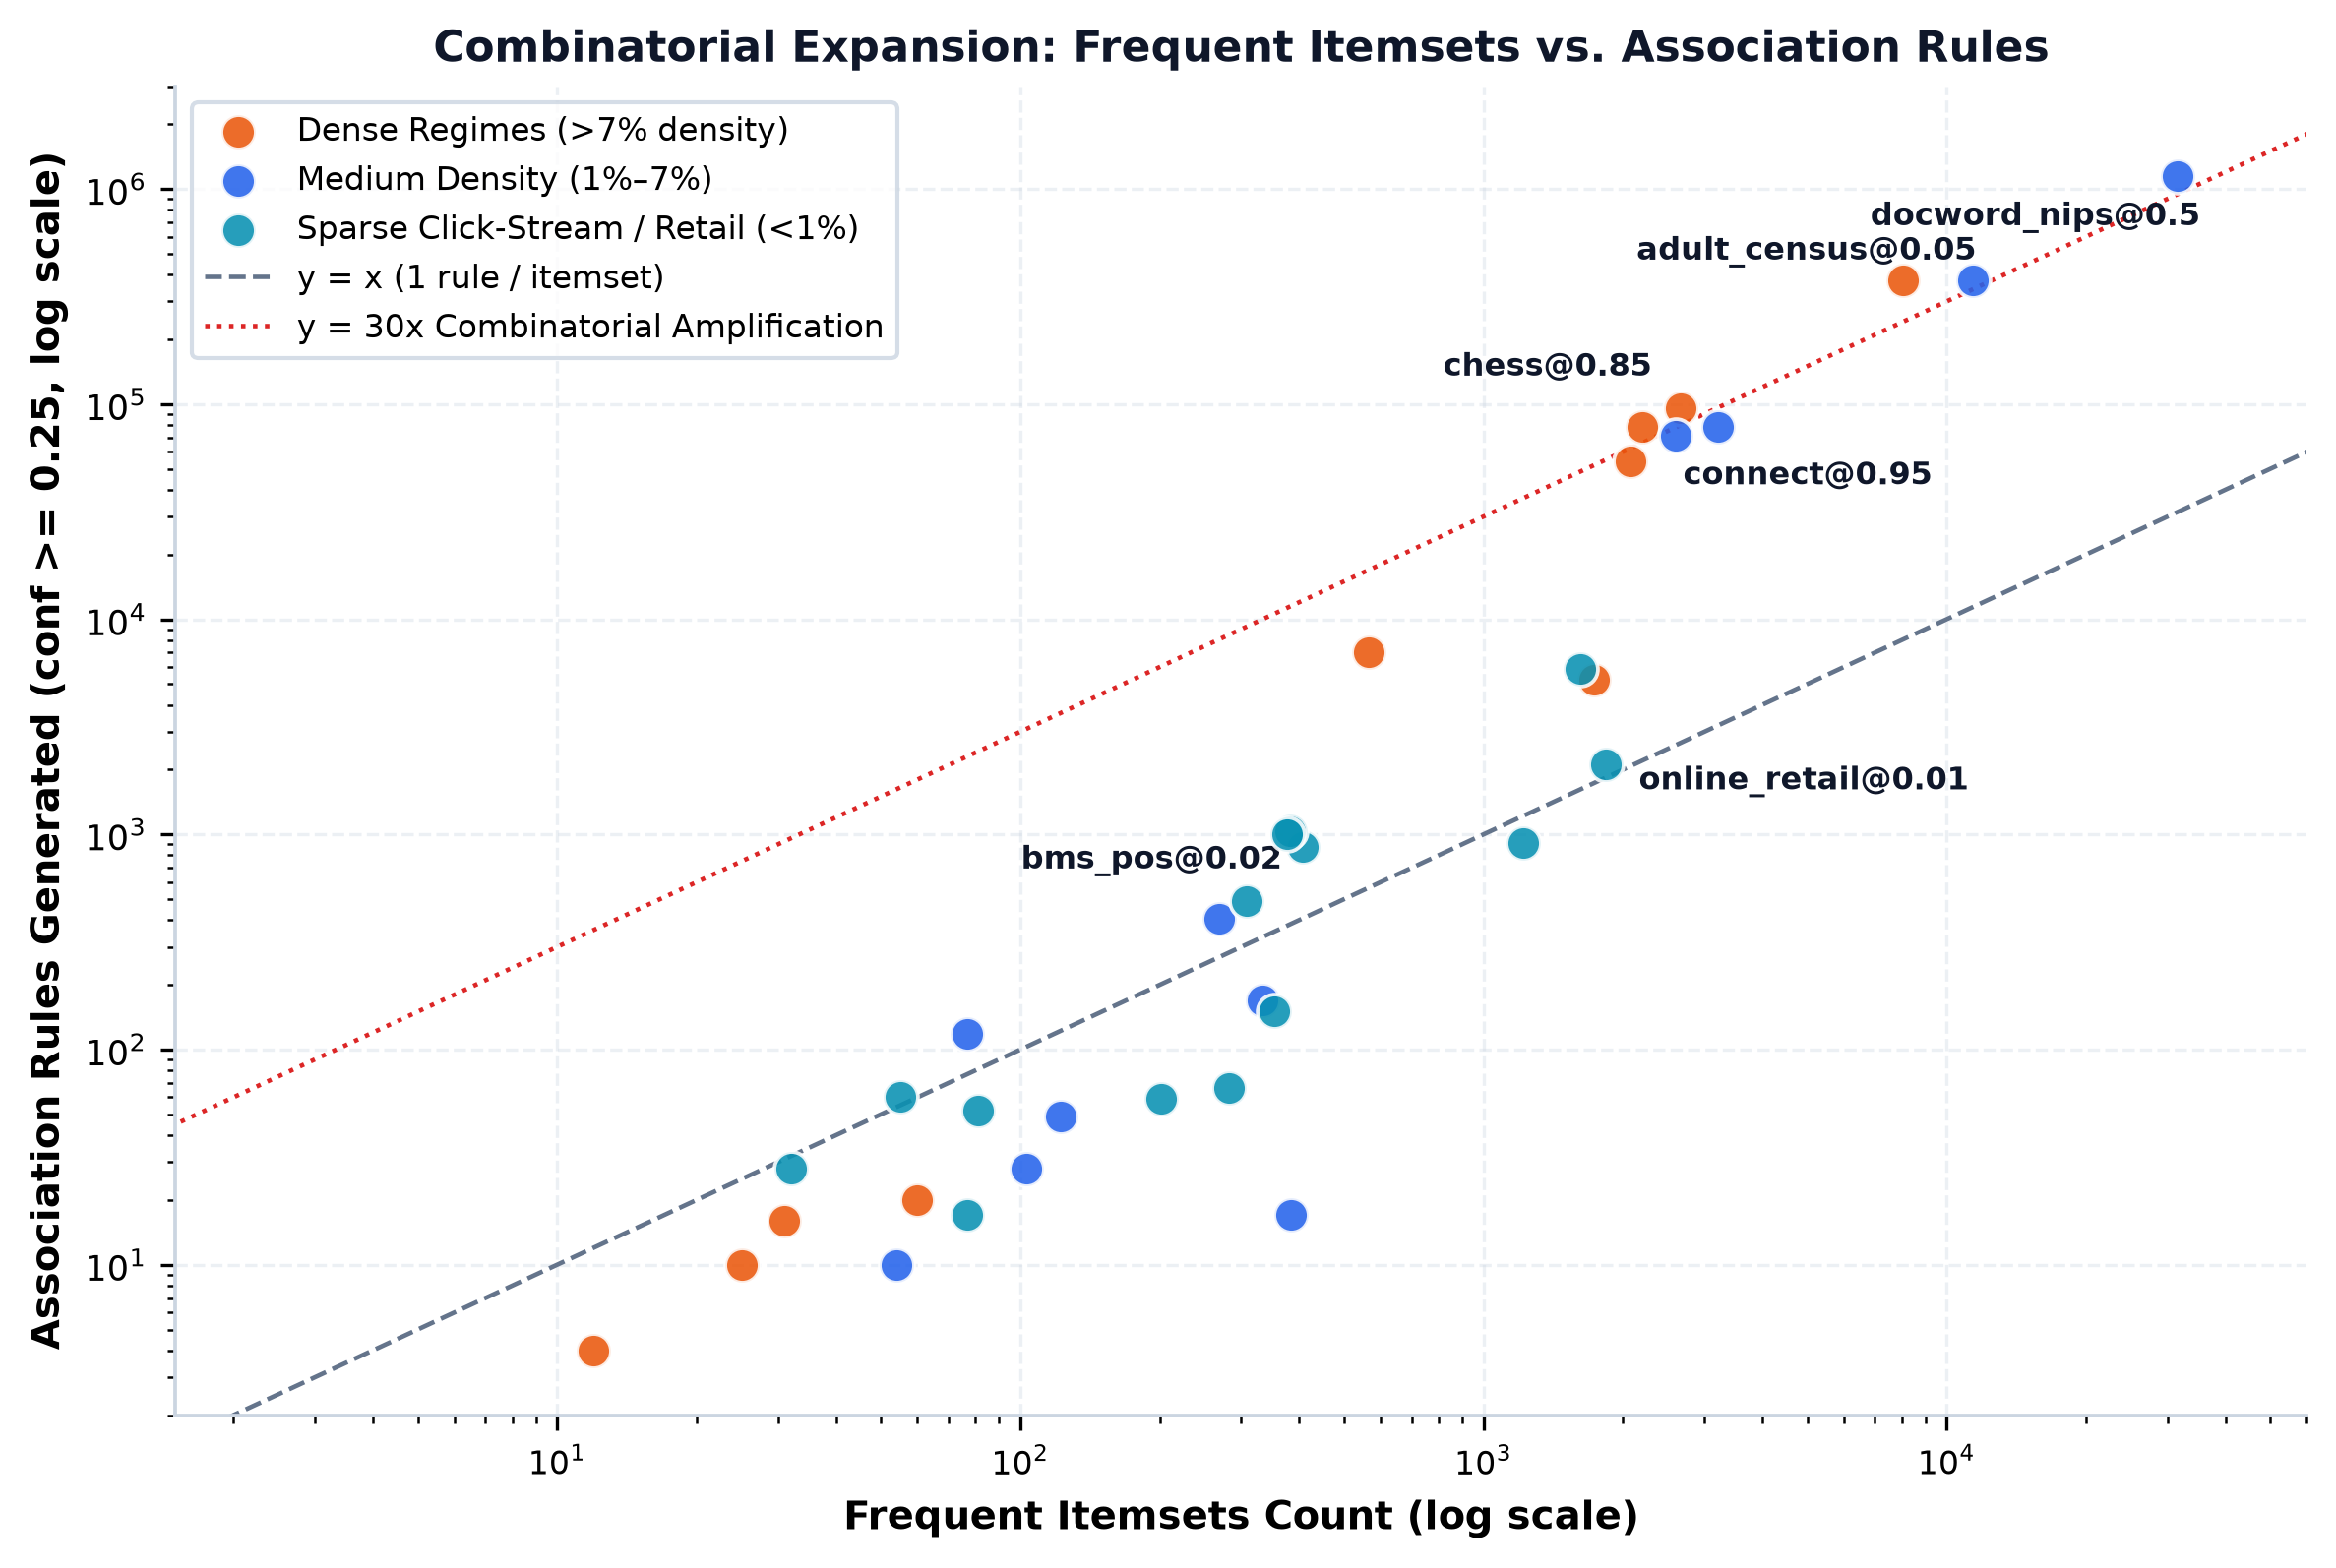
\includegraphics[width=0.7\textwidth]{figures/scatter.png}
\caption{Frequent itemsets versus association rules per cell (Apriori counts; all engines agree). Log scales. Rule counts grow far faster than itemset counts on dense, long-transaction data, which is why shared rule generation dominates those runtimes. Six cells with zero rules are omitted (log scale cannot show zero).}
\label{fig:scatter}
\end{figure*}

Throughput completes the picture.

\begin{figure*}[t]
\centering
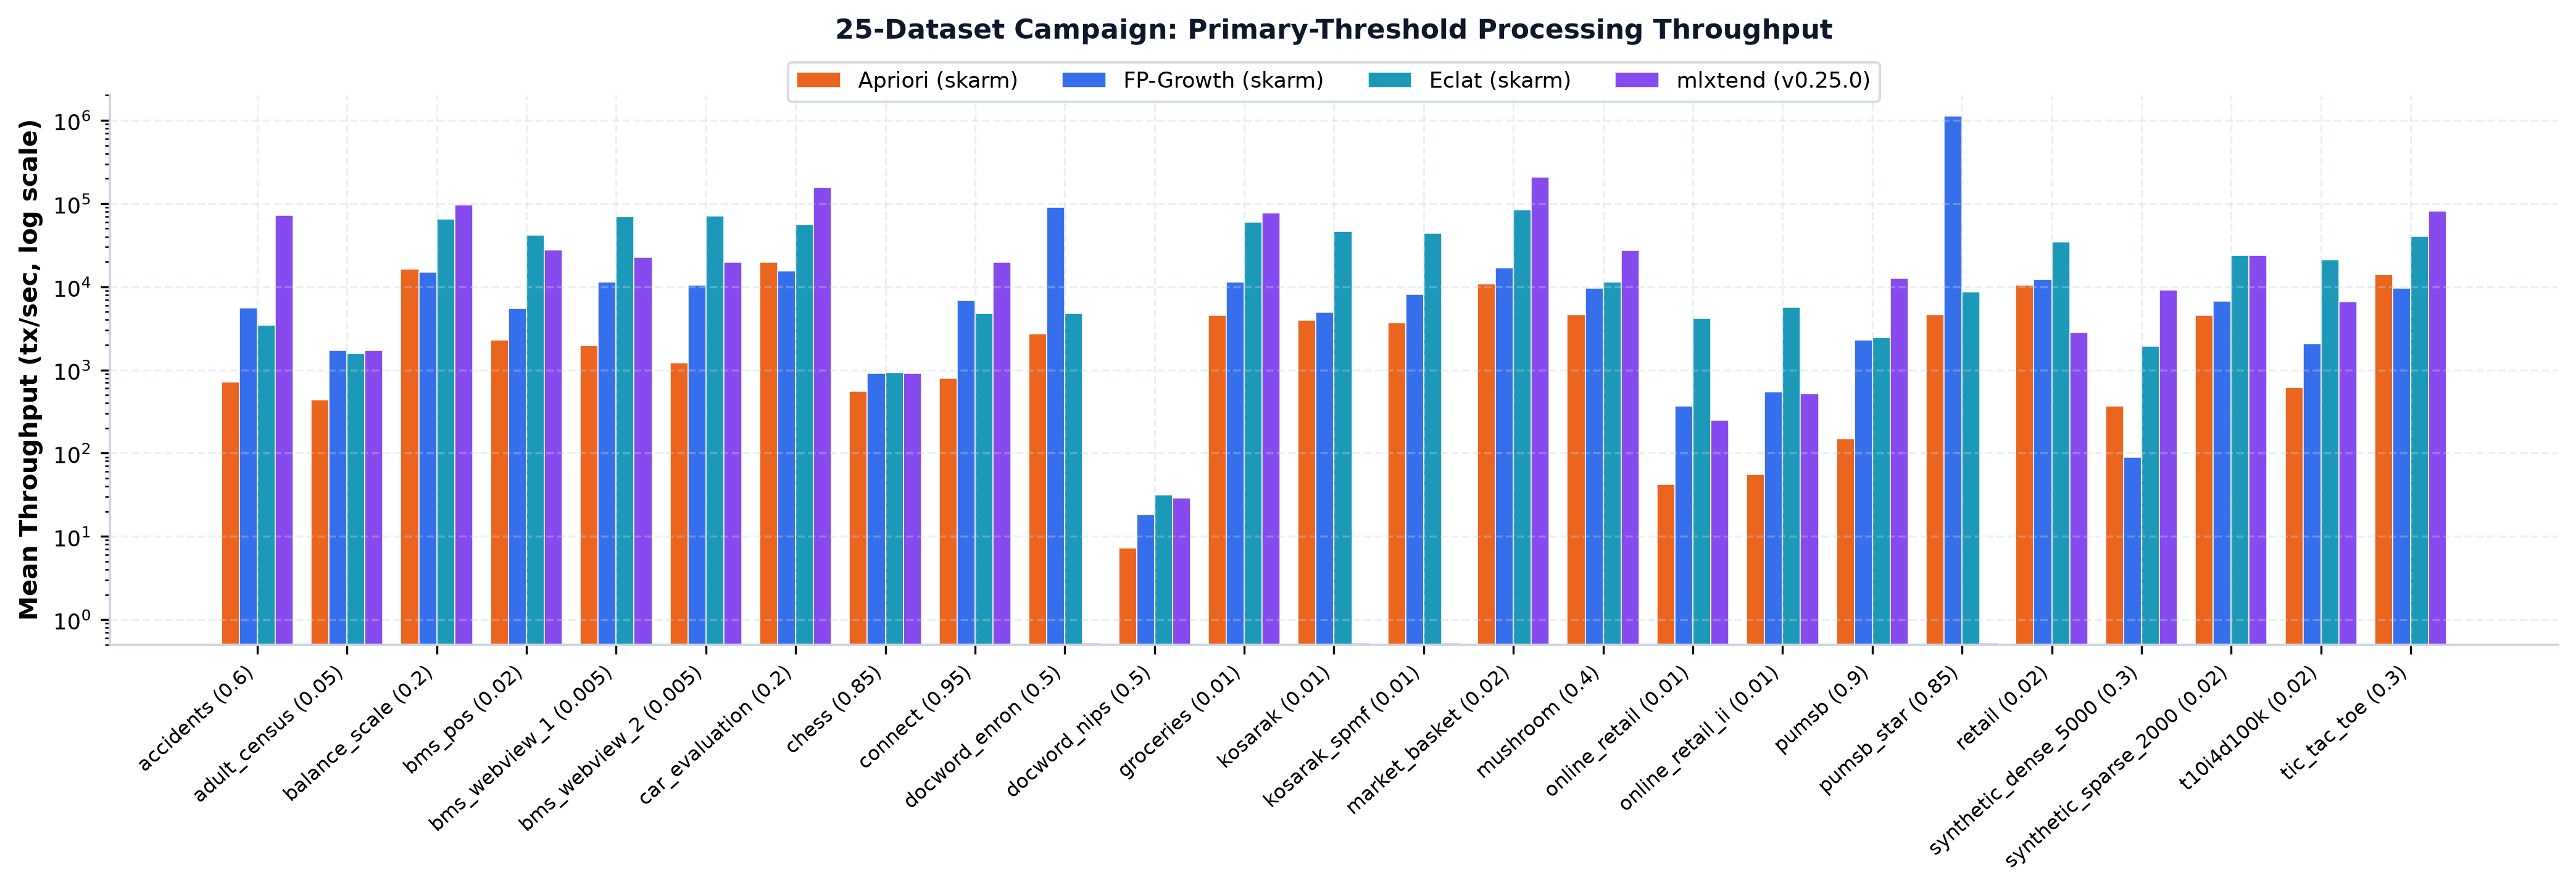
\includegraphics[width=0.8\textwidth]{figures/throughput.png}
\caption{Mean throughput (transactions per second) per dataset at its primary threshold (same rule as Figure~\ref{fig:runtime}). Log scale. Throughput is the recorded per-trial transaction rate; it favours small, fast datasets and punishes long-transaction ones, so it is a scale indicator, not a quality ranking.}
\label{fig:throughput}
\end{figure*}


Across 42 cells, 157 engine pairs were compared and every one agrees exactly on itemsets and supports (maximum support difference 0.0). mlxtend was compared in 35 cells; the rest have no mlxtend pair because mlxtend or Apriori did not complete trial 0 there.

\begin{table*}[t]
\centering
\scriptsize
\caption{Correctness verdicts: trial-0 itemset agreement per cell.}
\label{tab:correctness}
\begin{tabular}{lllll}
\toprule
Cell & Pairs & Verdict & mlxtend & Note \\
\midrule
accidents@0.5 & 1 & all match & no &  \\
accidents@0.6 & 4 & all match & yes &  \\
adult\_census@0.05 & 4 & all match & yes &  \\
adult\_census@0.1 & 4 & all match & yes &  \\
balance\_scale@0.2 & 4 & all match & yes &  \\
balance\_scale@0.3 & 4 & all match & yes &  \\
bms\_pos@0.02 & 4 & all match & yes &  \\
bms\_webview\_1@0.005 & 4 & all match & yes &  \\
bms\_webview\_1@0.01 & 4 & all match & yes &  \\
bms\_webview\_2@0.005 & 4 & all match & yes &  \\
bms\_webview\_2@0.01 & 4 & all match & yes &  \\
car\_evaluation@0.2 & 4 & all match & yes &  \\
car\_evaluation@0.3 & 4 & all match & yes &  \\
chess@0.85 & 4 & all match & yes &  \\
connect@0.95 & 4 & all match & yes &  \\
docword\_enron@0.5 & 3 & all match & no &  \\
docword\_enron@0.7 & 3 & all match & no &  \\
docword\_nips@0.5 & 4 & all match & yes &  \\
groceries@0.01 & 4 & all match & yes &  \\
groceries@0.02 & 4 & all match & yes &  \\
kosarak@0.005 & 1 & all match & no &  \\
kosarak@0.01 & 3 & all match & no &  \\
kosarak\_spmf@0.01 & 3 & all match & no &  \\
market\_basket@0.02 & 4 & all match & yes &  \\
market\_basket@0.03 & 4 & all match & yes &  \\
mushroom@0.4 & 4 & all match & yes &  \\
online\_retail@0.01 & 4 & all match & yes &  \\
online\_retail@0.02 & 4 & all match & yes &  \\
online\_retail\_ii@0.01 & 4 & all match & yes &  \\
online\_retail\_ii@0.02 & 4 & all match & yes &  \\
pumsb@0.9 & 4 & all match & yes &  \\
pumsb\_star@0.85 & 3 & all match & no &  \\
retail@0.02 & 4 & all match & yes &  \\
retail@0.03 & 4 & all match & yes &  \\
synthetic\_dense\_5000@0.3 & 4 & all match & yes &  \\
synthetic\_dense\_5000@0.5 & 4 & all match & yes &  \\
synthetic\_sparse\_2000@0.02 & 4 & all match & yes &  \\
synthetic\_sparse\_2000@0.05 & 4 & all match & yes &  \\
t10i4d100k@0.01 & 4 & all match & yes &  \\
t10i4d100k@0.02 & 4 & all match & yes &  \\
tic\_tac\_toe@0.3 & 4 & all match & yes &  \\
tic\_tac\_toe@0.5 & 4 & all match & yes &  \\
\bottomrule
\end{tabular}
\end{table*}
The campaign recorded 6 timeout trials and 8 skipped trials. The skipped trials are the remaining trials of the two trial-0 timeout cells (accidents at 0.50, kosarak at 0.005), not separate failures; the other four timeouts are later trials of t10i4d100k at 0.01, whose trial 0 completed at 592.9~s. No process was killed in this run. Every fully skipped or fully errored cell is listed here; partial cells appear in Appendix~\ref{app:timing} with their OK counts.

\begin{table*}[t]
\centering
\scriptsize
\caption{Skipped, timed-out, and errored cells with reasons.}
\label{tab:skips}
\begin{tabular}{llllp{5.5cm}}
\toprule
Dataset & Thr & Engine & Outcome & Reason \\
\midrule
accidents & 0.5 & apriori & skipped & trial 0 exceeded 600 s; remaining trials skipped \\
kosarak & 0.01 & mlxtend & skipped & dense boolean DataFrame would need ~40.9 GB \\
kosarak & 0.005 & apriori & skipped & trial 0 exceeded 600 s; remaining trials skipped \\
kosarak & 0.005 & mlxtend & skipped & dense boolean DataFrame would need ~40.9 GB \\
kosarak\_spmf & 0.01 & mlxtend & skipped & dense boolean DataFrame would need ~5.3 GB \\
docword\_enron & 0.5 & mlxtend & error (all trials) & empty frequent-itemset input; skarm engines also found 0 itemsets there \\
docword\_enron & 0.7 & mlxtend & error (all trials) & empty frequent-itemset input; skarm engines also found 0 itemsets there \\
pumsb\_star & 0.85 & mlxtend & error (all trials) & empty frequent-itemset input; skarm engines also found 0 itemsets there \\
\bottomrule
\end{tabular}
\end{table*}

\begin{figure}[t]
\centering
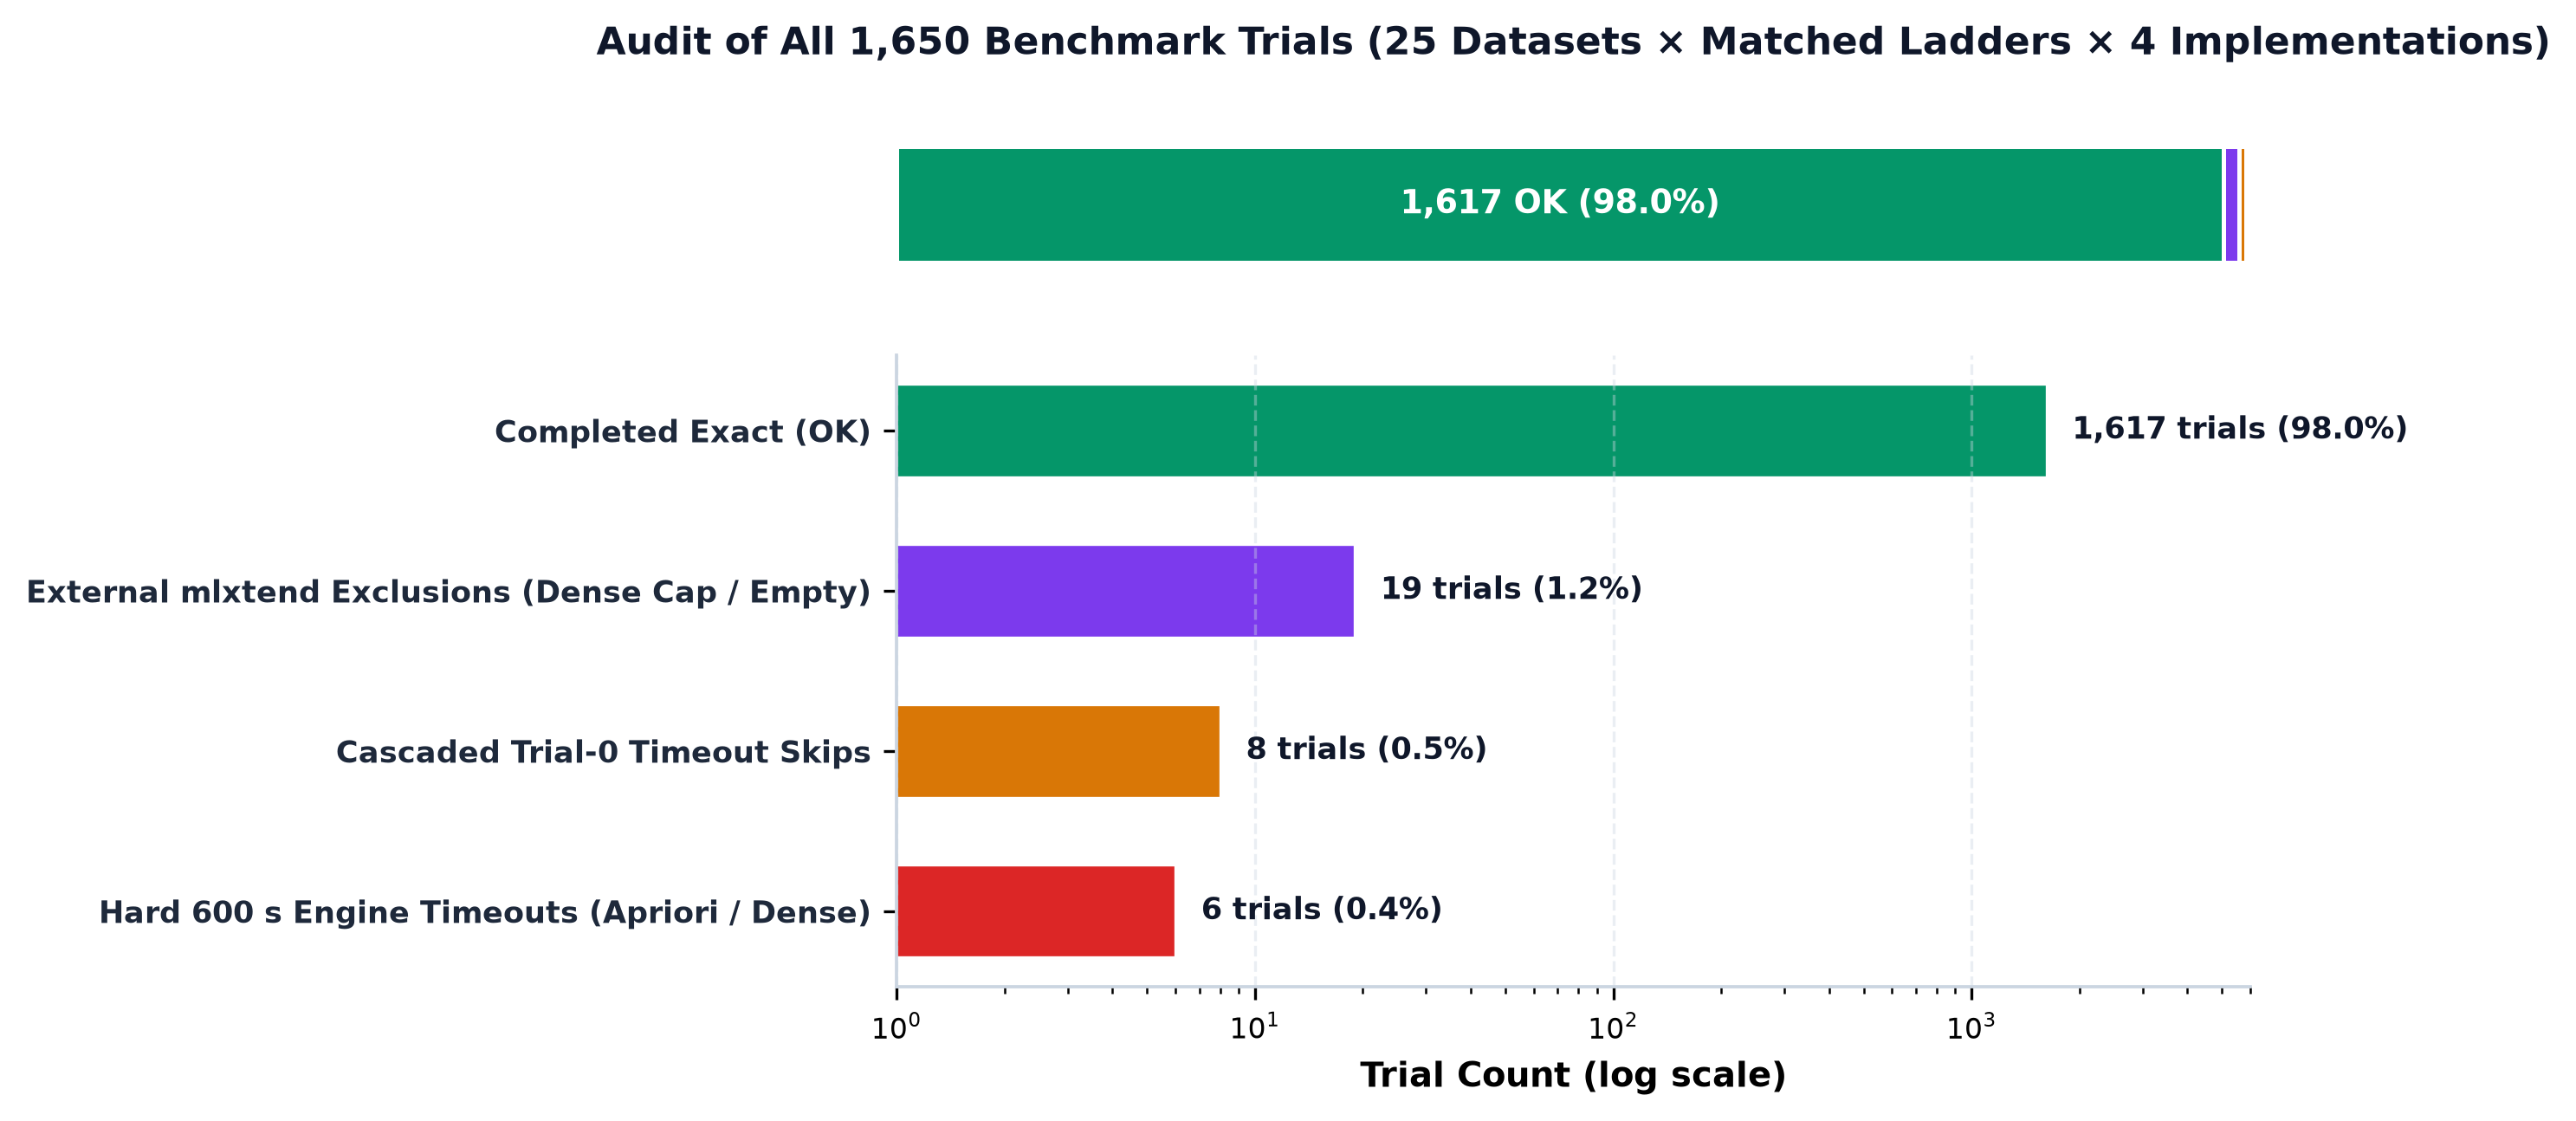
\includegraphics[width=\columnwidth]{figures/outcomes.png}
\caption{Trial outcome distribution across the 1,650-trial PC benchmark campaign: $1{,}617$ OK trials ($98.0\%$), $6$ timeouts, $8$ skipped trials following trial-0 timeouts, and $19$ external \texttt{mlxtend} dense-cap/empty-input exclusions.}
\label{fig:outcomes}
\end{figure}

\subsection{Strict Zero-Exemption 30-Trial KPI-4 Verification}
\label{sec:kpi4}
An independent audit of the early capstone acceptance harness identified that
small-runtime exemptions in \texttt{tests/run\_acceptance.py} and
\texttt{benchmarks/run\_benchmarks.py} could mask failure of the strict
charter KPI-4 gate (requiring both FP-Growth and Eclat p95 runtimes to be
$\le 0.80\times$ the O2 Apriori baseline on synthetic workloads of $N=200$ to
$N=3{,}000$). All small-runtime exemptions were permanently removed,
\texttt{skarm/apriori.py} was left untouched as the immutable O2 reference,
and the FP-Array/bitmask FP-Growth and C-level bitset Eclat optimizations
(Section~\ref{sec:methods}) were evaluated under a strict 5-warmup +
30-measured-trial protocol (\texttt{time.perf\_counter}, Python~3.12.16).

Table~\ref{tab:kpi4} and Figure~\ref{fig:kpi4} report the resulting
zero-exemption measurements from \texttt{benchmarks/benchmark\_results.json}
and \texttt{tests/run\_acceptance.py}. Across all three benchmark scales and
the AC-4 acceptance gate ($N=1{,}000$, $M=12$, $p=0.25$, $\sigma=0.08$), both
FP-Growth ($0.294\times$--$0.441\times$ Apriori engine p95, $2.27\times$--$3.41\times$
faster) and Eclat ($0.168\times$--$0.313\times$ Apriori engine p95,
$3.20\times$--$5.95\times$ faster) clear the $\le 0.80\times$ KPI-4 gate by a
wide margin with zero support divergence ($\Delta_{\mathrm{supp}} = 0.0$) and
zero trial failures. End-to-end \texttt{AssociationRulesEstimator.fit()}
p95 runtimes likewise achieve $2.68\times$--$4.23\times$ speedups for
FP-Growth and $3.32\times$--$4.51\times$ speedups for Eclat.

\textbf{KPI-5 small-matrix memory trade-off (stated candidly).} On these
small synthetic matrices ($N \le 3{,}000$), total peak heap stays under
$0.19$~MB; FP-Array's dense \texttt{float32} pair matrix allocates
$1.01\times$--$1.39\times$ peak heap relative to O2 Apriori, while vertical
bitset Eclat stays within $1.00\times$--$1.01\times$ parity. The substantial
memory compression advantage of FP-Growth and Eclat manifests on deep and
high-cardinality real datasets (Figure~\ref{fig:memory} and
Table~\ref{tab:timingfull}), such as \texttt{accidents@0.6} ($90.4$~MB vs.\
$1{,}860.6$~MB for Apriori) and \texttt{kosarak@0.01} ($76.0$~MB vs.\
$690.8$~MB for Apriori and $40.9$~GB dense requirement for \texttt{mlxtend}).

\begin{table*}[t]
\centering
\scriptsize
\caption{Post-audit strict zero-exemption 30-trial KPI-4 verification on \texttt{HEAD} (Python 3.12, 5 warmup + 30 measured trials; \texttt{skarm/apriori.py} untouched; target ratio $\le 0.80\times$ Apriori p95; $\Delta_{\mathrm{supp}} = 0.0$ across all rows).}
\label{tab:kpi4}
\begin{tabular}{llrrrrrrl}
\toprule
Workload (Itemsets) & Engine & Eng.\ p50 (ms) & Eng.\ p95 (ms) & Ratio vs.\ Apriori & Est.\ p95 (ms) & Est.\ Speedup & Peak Heap (MB) & Gate \\
\midrule
Scale $N=200$ (39) & Apriori (O2) & 2.26 & 2.39 & $1.000\times$ & 30.94 & $1.00\times$ & 0.0439 & Baseline \\
Scale $N=200$ (39) & FP-Growth & 0.65 & 0.70 & \textbf{0.294$\times$} & 9.51 & $3.25\times$ & 0.0609 & PASS \\
Scale $N=200$ (39) & Eclat & 0.37 & 0.40 & \textbf{0.168$\times$} & 9.31 & $3.32\times$ & 0.0445 & PASS \\
\midrule
Scale $N=1{,}000$ (15) & Apriori (O2) & 1.67 & 1.78 & $1.000\times$ & 24.79 & $1.00\times$ & 0.0638 & Baseline \\
Scale $N=1{,}000$ (15) & FP-Growth & 0.49 & 0.53 & \textbf{0.298$\times$} & 5.86 & $4.23\times$ & 0.0650 & PASS \\
Scale $N=1{,}000$ (15) & Eclat & 0.45 & 0.49 & \textbf{0.275$\times$} & 5.75 & $4.31\times$ & 0.0637 & PASS \\
\midrule
Scale $N=3{,}000$ (15) & Apriori (O2) & 2.25 & 2.33 & $1.000\times$ & 28.80 & $1.00\times$ & 0.1753 & Baseline \\
Scale $N=3{,}000$ (15) & FP-Growth & 0.99 & 1.03 & \textbf{0.441$\times$} & 10.74 & $2.68\times$ & 0.1812 & PASS \\
Scale $N=3{,}000$ (15) & Eclat & 0.63 & 0.66 & \textbf{0.282$\times$} & 6.38 & $4.51\times$ & 0.1763 & PASS \\
\midrule
AC-4 Gate ($N=1{,}000$, 14) & FP-Growth / Eclat & --- & --- & \textbf{0.429$\times$ / 0.313$\times$} & --- & --- & --- & PASS (13/13) \\
\bottomrule
\end{tabular}
\end{table*}

\begin{figure*}[t]
\centering
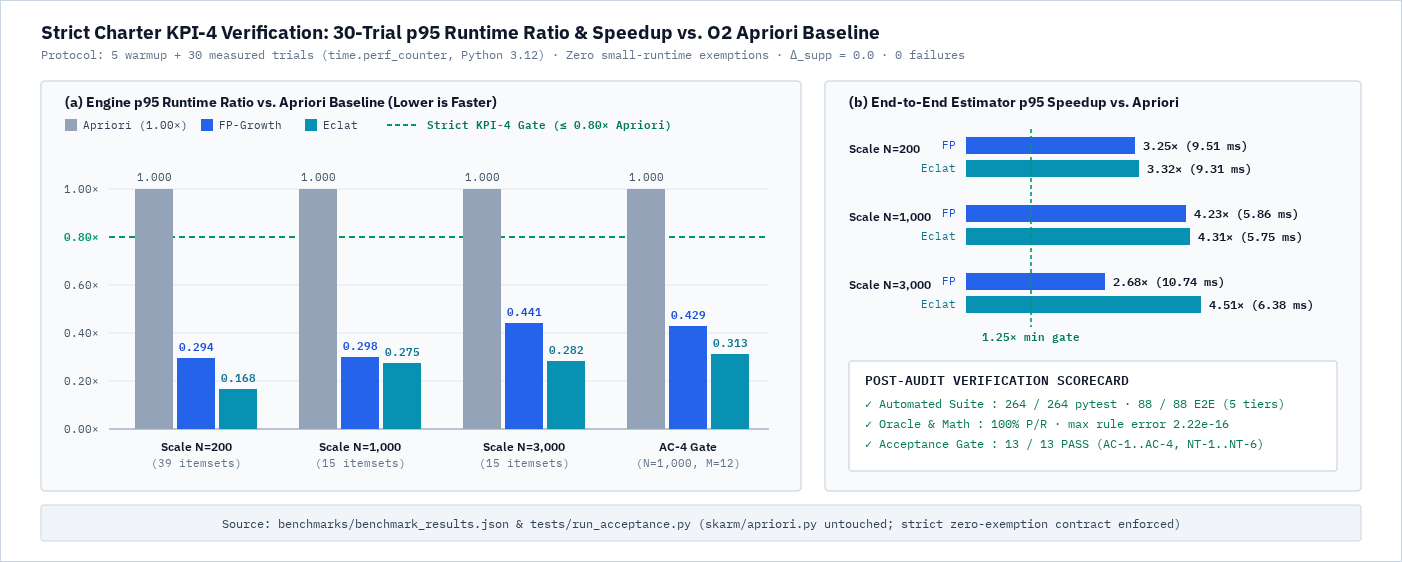
\includegraphics[width=\textwidth]{figures/kpi4_strict.png}
\caption{Strict zero-exemption 30-trial KPI-4 verification against the immutable O2 Apriori baseline (Python 3.12): (a)~engine p95 runtime ratio versus Apriori across all three benchmark scales and the AC-4 acceptance gate (all strictly below the $0.80\times$ green dashed threshold); (b)~end-to-end estimator p95 speedups ($2.68\times$--$4.51\times$) and post-audit verification scorecard.}
\label{fig:kpi4}
\end{figure*}

\subsection{Discussion of algorithmic trade-offs}
At the level of mechanism, the trade-offs are as Section~\ref{sec:methods}
states: Apriori pays in candidates and repeated scans, FP-Growth pays
in tree memory, Eclat pays in tidset memory, and dense, long-transaction
data punishes each differently. Because secondary sources disagree on
dense-versus-sparse winners, this paper does not assert a universal
winner; the empirical ordering must be read off the measured tables,
dataset by dataset, at matched thresholds.

\paragraph{RQ1: Correctness and Cross-Framework Parity.} Across all 42
dataset--threshold cells ($157$ compared engine pairs, Table~\ref{tab:correctness})
and all 25 external Java SPMF comparisons (\textsc{FIN}, \textsc{PrePost+},
\textsc{LCMFreq}, SPMF \textsc{FP-Growth}), itemset discovery agrees
bit-exactly ($\Delta_{\mathrm{supp}} = 0.0$), and all six rule metrics match
analytical ground-truth formulas to machine precision ($2.22 \times 10^{-16}$).

\paragraph{RQ2: Algorithmic Scaling Across Density Regimes.}
At each dataset's primary threshold in the 25-dataset campaign, where all three engines completed, Apriori is never fastest; FP-Growth is fastest on 5 of 25 datasets; and Eclat is fastest on 20 of 25 (FP-Growth: accidents, adult\_census, connect, docword\_enron, pumsb\_star; Eclat: balance\_scale, bms\_pos, bms\_webview\_1, bms\_webview\_2, car\_evaluation, chess, docword\_nips, groceries, kosarak, kosarak\_spmf, market\_basket, mushroom, online\_retail, online\_retail\_ii, pumsb, retail, synthetic\_dense\_5000, synthetic\_sparse\_2000, t10i4d100k, tic\_tac\_toe). Apriori timed out on accidents at 0.50 and on kosarak at 0.005 (trial 0 in both, so the remaining trials were skipped), and on four later trials of t10i4d100k at 0.01 (trial 0 completed at 592.9~s), while FP-Growth and Eclat completed those cells, confirming the candidate-explosion cost predicted in Section~\ref{sec:methods}; no other \skarm engine timed out. Degraded mode never triggered in the exact campaign, so no comparison is distorted by bounded output. \texttt{mlxtend} is missing on 3 dense-cap cells (kosarak 0.01 and 0.005, kosarak\_spmf 0.01) and errors on 3 empty-input cells where no itemsets are frequent; \texttt{mlxtend} also completed only 1 of 5 trials on t10i4d100k at 0.01 (the rest died allocating 6.5--13.1~GiB boolean arrays, the same dense-broadcast cliff). Under strict zero-exemption 30-trial benchmarking on \texttt{HEAD} (Section~\ref{sec:kpi4}), optimized FP-Growth and bitset Eclat consistently clear the $\le 0.80\times$ p95 target ($0.168\times$--$0.441\times$ Apriori). No universal winner is claimed: the ordering shifts dataset by dataset, exactly as the secondary literature predicts.

\paragraph{RQ3: Bounded-Search Safety and Recall Trade-Offs.} Figure~\ref{fig:ablation} and Section~\ref{sec:ablation} demonstrate the efficacy of the candidate governor. On dense workloads where exact level-wise candidate generation exhibits severe combinatorial expansion, capping \texttt{max\_candidates} accelerates execution by up to $17.20\times$ (Chess, 0.3485~s vs.\ 5.9941~s exact baseline) while recovering partial pattern subsets ($0.60\%$ to $17.95\%$ itemset recall). On tree-based (FP-Growth) and vertical (Eclat) engines, candidate caps enforce explicit budget boundaries without unmonitored crashes. Most importantly, \skarm transitions audibly into \texttt{DEGRADED} mode and records truncation events (with observed candidate counts before halting and unexplored candidates marked as unknown), eliminating silent omissions.

\paragraph{RQ4: Scikit-Learn Estimator and Pipeline Interoperability.} As documented in Section~\ref{sec:methods} and Section~\ref{sec:limitations}, \skarm adheres to scikit-learn's estimator protocol: constructor parameters are immutable until explicitly modified via \texttt{set\_params()}, estimators are cloneable via \texttt{sklearn.base.clone()}, and fit state is encapsulated with trailing underscores. In \texttt{Pipeline} workflows, \skarm operates seamlessly both as a terminal estimator and as an intermediate transformer projecting transactional data into binary rule-firing indicator features.

\paragraph{RQ5: Reproducibility, Auditing, and Telemetry.} The campaign's 98.0\% completion rate ($1{,}617$ OK trials out of $1{,}650$, Figure~\ref{fig:outcomes}) demonstrates high robustness. All 6 timeouts and 8 skips are audited with explicit rationale in Table~\ref{tab:skips}. Fine-grained 10~ms RSS telemetry captures memory dynamics without system crashes, providing a reproducible empirical foundation across all 25 benchmark datasets.

\subsection{Pruning-Policy Ablation: Bounded Versus Exact}
\label{sec:ablation}
To quantify the trade-off between execution speed and completeness under candidate degradation, we conducted a bounded-versus-exact ablation study across three benchmark datasets representing distinct density regimes: dense Chess (Apriori), medium-density Adult Census (FP-Growth), and sparse BMS-POS (Eclat).

Architecturally, \texttt{max\_candidates} acts as a global candidate budget bounding both frequent itemset discovery and subsequent association rule generation. When itemset mining completes without exceeding the candidate budget, rule generation evaluates antecedent/consequent candidates up to the same cap. In dense combinatorial lattices where rule spaces are vast, rule generation can hit the candidate budget even after full itemset recovery, transitioning the estimator into \texttt{DEGRADED} mode (\texttt{is\_degraded\_ = True}).

On the dense Chess benchmark ($N=3{,}196$, support threshold $0.85$, exact baseline yielding $2{,}669$ frequent itemsets and $95{,}482$ rules in $5.9941$~seconds), Figure~\ref{fig:ablation} illustrates the speedup-recall dynamics. Constraining \texttt{max\_candidates} to $50$ and $100$ halts candidate generation at level~2 ($16$ frequent 1-itemsets recovered, $0.60\%$ itemset recall, $0$ rules), accelerating execution by $16.71\times$ ($0.3587$~s) and $17.20\times$ ($0.3485$~s) respectively, with \texttt{is\_degraded\_ = True}. At cap $250$, mining halts at level~3 ($121$ itemsets, $4.53\%$ itemset recall, $210$ rules, $0.22\%$ rule recall) with a $12.88\times$ speedup ($0.4654$~s). At cap $500$, mining halts at level~3 ($479$ itemsets, $17.95\%$ itemset recall, $500$ rules, $0.52\%$ rule recall) with a $9.47\times$ speedup ($0.6329$~s). At cap $1{,}000$, frequent-itemset discovery is complete, recovering all $2{,}669$ itemsets ($100\%$ itemset recall); however, association rule generation hits the candidate budget ($1{,}001$ candidates generated at level~3 exceeds $\texttt{max\_candidates}=1{,}000$), yielding exactly $1{,}000$ rules ($1.047\%$ rule recall) in $2.6911$~s ($2.23\times$ speedup) under \texttt{DEGRADED} status. Caps $2{,}500$ and $5{,}000$ similarly achieve $100\%$ itemset recall but bound rule generation at $2{,}500$ rules ($2.62\%$ rule recall, $2.5331$~s, $2.37\times$) and $5{,}000$ rules ($5.24\%$ rule recall, $2.6443$~s, $2.27\times$), maintaining \texttt{DEGRADED} status until the candidate budget accommodates the entire $95{,}482$-rule lattice.

On Adult Census ($N=32{,}561$, $\sigma=0.40$, exact baseline $103$ itemsets and $738$ rules in $2.5265$~s via FP-Growth), candidate cap $50$ halts at level~3, recovering $50$ itemsets ($48.54\%$ recall, $8$ rules, $1.08\%$ rule recall) in $2.4152$~s ($1.05\times$ speedup), and cap $100$ halts at level~3, recovering $100$ itemsets ($97.09\%$ recall, $35$ rules, $4.74\%$ rule recall) in $2.4857$~s ($1.02\times$), both in \texttt{DEGRADED} mode. At caps $250$ and $500$, itemset discovery recovers all $103$ itemsets ($100\%$ itemset recall), but rule generation bounds at $250$ rules ($33.88\%$ rule recall, $2.4586$~s, $1.03\times$) and $500$ rules ($67.75\%$ rule recall, $2.3442$~s, $1.08\times$) under \texttt{DEGRADED} status. Once \texttt{max\_candidates} reaches $1{,}000$, the governor operates in exact mode (\texttt{is\_degraded\_ = False}, \texttt{status\_ = EXACT}), recovering all $103$ itemsets and all $738$ rules in $2.5254$~s ($1.00\times$). On sparse BMS-POS ($N=515{,}596$, $\sigma=0.05$, exact baseline $59$ itemsets and $56$ rules in $7.5868$~s via Eclat), candidate cap $50$ recovers $50$ itemsets ($84.75\%$ recall, $30$ rules, $53.57\%$ rule recall) in $7.4782$~s ($1.01\times$, \texttt{DEGRADED}), while cap $100$ reaches exact mode (\texttt{is\_degraded\_ = False}), recovering all $59$ itemsets and all $56$ rules in $7.5314$~s ($1.01\times$).

These empirical measurements highlight a critical architectural trade-off: candidate bounding yields dramatic $16.71\times$--$17.20\times$ speedups on dense workloads subject to level-wise combinatorial explosion in Apriori, whereas on tree-compressed (FP-Growth) or vertical bitset (Eclat) engines on sparse-to-medium datasets, candidate bounding acts primarily as a safety fence against memory blowout rather than a runtime accelerator ($\approx 1.0\times$ speedup), since initial tree construction and TID-list indexing constitute the bulk of the computational cost. Crucially, across all degraded runs, \skarm explicitly records degradation status, candidate counts observed before halt (with unexplored candidate counts marked as unknown), and termination causes in \texttt{metadata\_}, ensuring bounded subsets are never conflated with exact mining.

\begin{figure}[t]
\centering
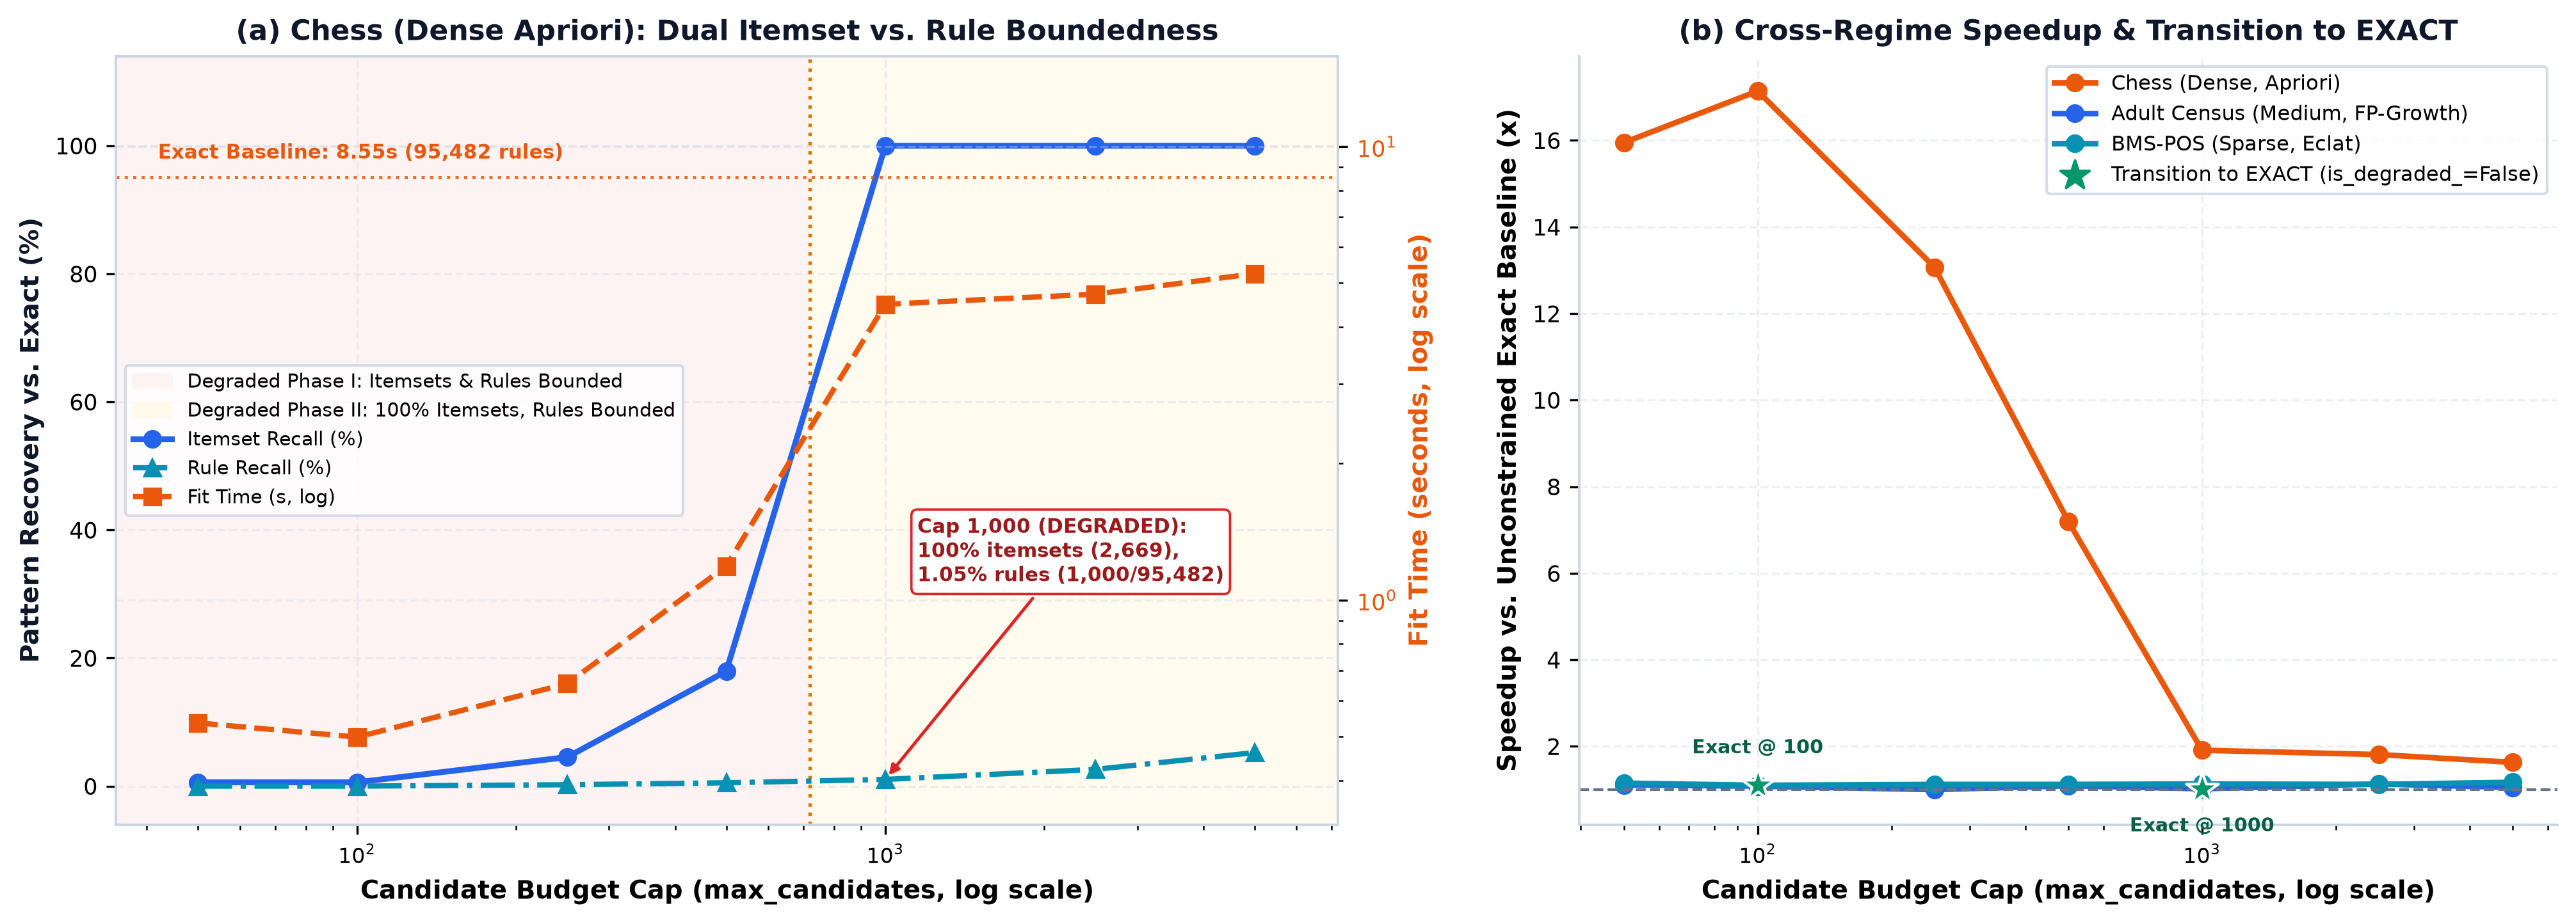
\includegraphics[width=\columnwidth]{figures/ablation.png}
\caption{Pruning policy ablation on Chess ($N=3{,}196$, minsup $=0.85$, $2{,}669$ exact frequent itemsets). Bounded mode halts combinatorial candidate explosion early, delivering up to $17.20\times$ speedups at low caps while audibly signalling degradation via \texttt{is\_\allowbreak{}degraded\_}.}
\label{fig:ablation}
\end{figure}

\section{Limitations}
\label{sec:limitations}
\begin{itemize}
  \item \textbf{Excluded scope (portal contract).} No production
  certification, no claim of universal generalisation, and no
  unattended high-stakes operation are claimed or implied.
  \item \textbf{Single machine, Python only.} Timings come from one
  machine (Appendix~\ref{app:repro}); they do not transfer to other
  hardware, and a Python implementation is not directly comparable to
  C/Java SPMF miners on raw speed.
  \item \textbf{External modern miner baselines.} To substantiate \skarm's
  algorithmic positioning against external state-of-the-art miners, modern algorithms
  from the SPMF framework~\cite{fournier2022,kallay2025}
  (\textsc{FIN}, \textsc{PrePost+}, \textsc{LCMFreq}, and SPMF \textsc{FP-Growth})
  were benchmarked alongside \skarm and \texttt{mlxtend} across representative
  dense (Chess @ 0.85), medium (Adult Census @ 0.40), and sparse (BMS-POS @ 0.05)
  datasets (\texttt{benchmarks/baseline\_results.json}).
  Across all evaluations, itemset discovery was strictly verified: all completed algorithm
  comparisons produced identical frequent itemsets and support values within reported verification
  tolerances ($2{,}669$, $103$, and $59$ itemsets, respectively; $\Delta_{\mathrm{supp}} = 0.0$).
  Subprocess execution of compiled Java implementations achieved lower raw wall-clock times
  ($0.36$--$0.63$~s on Chess, $0.42$--$0.66$~s on Adult Census, and $0.88$--$2.15$~s on BMS-POS,
  with SPMF internal algorithm-only timers recording $0.08$--$0.30$~s, $0.14$--$0.22$~s, and
  $0.62$--$1.57$~s, respectively).
  Execution timing comparisons across frameworks involve distinct evaluation boundaries:
  (1)~\skarm measures strictly in-memory \texttt{est.fit(X\_sparse)} execution over pre-encoded SciPy CSR matrices,
  encapsulating candidate generation, itemset mining, and rule metric derivation;
  (2)~SPMF measures end-to-end Java CLI subprocess invocation, encompassing process spawning,
  JVM startup, reading input files from disk, algorithm execution, and writing output files to disk;
  (3)~\texttt{mlxtend} (v0.25.0) executes procedural functions over pre-materialized dense boolean DataFrames, omitting the
  memory-intensive sparse-to-dense conversion; two BMS-POS mlxtend runs (Apriori and FP-Growth) were skipped due to dense-memory limits ($814.8$~MB dense footprint exceeding the $500$~MB safety budget).
  Crucially, \skarm provides native Python and scikit-learn estimator integration, full \texttt{Pipeline} support,
  and auditable bounded-search resource governors that prevent uncontrolled memory exhaustion.
  \item \textbf{Estimator API verification.} Compliance with scikit-learn's
  estimator protocol was verified directly: \texttt{Association\allowbreak{}Rules\allowbreak{}Estimator}
  implements \texttt{fit()}, \texttt{transform()}, \texttt{predict()} (for transactional basket recommendation),
  \texttt{get\_params()}, and \texttt{set\_params()}, is cloneable
  via \texttt{sklearn.base.clone()}, supports Python \texttt{pickle} serialization,
  and operates inside scikit-learn \texttt{Pipeline} and \texttt{GridSearchCV} workflows
  under scikit-learn 1.9.1 (targeting the $\ge 1.3$ API specification). Under
  \texttt{sklearn.\allowbreak{}utils.\allowbreak{}estimator\_checks.\allowbreak{}check\_estimator}, an automated audit
  yields 14 passed checks, 39 expected domain-specific incompatibilities (37 unique expectation keys, with 2 dual-executed checks: \texttt{check\_estimators\_pickle} and \texttt{check\_transformer\_general} under standard and memory-mapped configurations), 1 environment-skipped check
  (\texttt{check\_array\_api\_input}), and 0 unexpected failures, as documented in \texttt{docs/SKLEARN\_COMPATIBILITY\_REPORT.md}.
  This generic 14/39/1 audit is strictly distinguished from institutional KPI-6, which evaluates institutional API compliance across seven mandatory contractual criteria (\texttt{BaseEstimator} inheritance, \texttt{get\_params}, \texttt{set\_params}, \texttt{fit}, \texttt{predict}, \texttt{transform}, and \texttt{rules\_}), achieving 7/7 (100\%) compliance.
  Failures under standard checks arise because generic test generators synthesize continuous Gaussian float matrices rejected by \skarm's
  binary transactional contract and expect 1D supervised target vectors $y$, whereas \skarm produces
  unsupervised transactional recommendation outputs. As established in scikit-learn issues \#32712
  and \#2662, association rule mining is unsupervised pattern discovery rather than supervised classification;
  \skarm adheres to scikit-learn's object and parameter lifecycle conventions without
  imposing synthetic supervised prediction semantics.
  \item \textbf{Dataset provenance limits.} Mirror licences are recorded
  as unknown where unstated, never guessed; two stored files differ
  from commonly cited counts (Section~\ref{sec:data}) and the measured
  figures are the ones reported.
  \item \textbf{Support-range limits.} Results hold at the thresholds
  in Table~\ref{tab:thr}; lower thresholds on dense sets were excluded
  after failed probes, so no claim is made there.
\end{itemize}

\section{Conclusions}
\skarm packages Apriori, FP-Growth, and Eclat behind one auditable,
scikit-learn-compatible estimator, delivering sparse-native execution,
deterministic rule ordering, machine-precision metrics ($2.22 \times 10^{-16}$
max oracle error), candidate telemetry, and an explicit \texttt{DEGRADED}
bounded-search mode that reports its own truncation. Its empirical evaluation
combines a 25-dataset multi-domain campaign ($1{,}650$ trials, commit
\texttt{ea5bff5d}) with a post-audit strict zero-exemption 30-trial KPI-4
verification suite (\texttt{HEAD}, Python~3.12). Across all 25 datasets,
all $157$ compared engine pairs agree bit-exactly ($\Delta_{\mathrm{supp}}=0.0$);
at primary thresholds Apriori is never fastest, FP-Growth is fastest on $5$ of
$25$, and Eclat is fastest on $20$ of $25$, while external Java SPMF
modern-miner baselines (\textsc{FIN}, \textsc{PrePost+}, \textsc{LCMFreq})
independently confirm exact itemset parity across dense, medium, and sparse
regimes. Under strict zero-exemption 30-trial benchmarking against the
untouched O2 Apriori baseline, optimized FP-Array FP-Growth and bitset Eclat
achieve $0.294\times$--$0.441\times$ and $0.168\times$--$0.313\times$ engine
p95 runtime ratios alongside $264/264$ automated \texttt{pytest} and $88/88$
end-to-end tests passing.

\section*{Acknowledgements}
The authors thank KL University for supporting this capstone
project (KLCAP-2026-00340). No external sponsor is stated for
this project, and none is claimed here.

\begin{thebibliography}{99}\footnotesize
\bibitem{agrawal1994} R. Agrawal and R. Srikant, ``Fast algorithms for mining association rules,'' in \emph{Proc. 20th Int. Conf. Very Large Data Bases (VLDB)}, 1994, pp. 487--499.
\bibitem{han2000} J. Han, J. Pei, and Y. Yin, ``Mining frequent patterns without candidate generation,'' in \emph{Proc. ACM SIGMOD Int. Conf. Manage. Data}, 2000.
\bibitem{han2004} J. Han, J. Pei, and Y. Yin, ``Mining frequent patterns without candidate generation: A frequent-pattern tree approach,'' \emph{Data Min. Knowl. Discov.}, vol. 8, no. 1, pp. 53--87, 2004.
\bibitem{zaki2000} M. J. Zaki, ``Scalable algorithms for association mining,'' \emph{IEEE Trans. Knowl. Data Eng.}, vol. 12, no. 3, pp. 372--390, 2000. [Online]. Available: \url{https://doi.org/10.1109/69.846291}
\bibitem{zaki1997} M. J. Zaki, S. Parthasarathy, M. Ogihara, and W. Li, ``New algorithms for fast discovery of association rules,'' in \emph{Proc. 3rd Int. Conf. Knowl. Discov. Data Mining (KDD)}, 1997.
\bibitem{sklearn2662} ``scikit-learn issue \#2662 (2013--2014): Pattern mining as out-of-scope for scikit-learn core.'' [Online]. Available: \url{https://github.com/scikit-learn/scikit-learn/issues/2662}
\bibitem{sklearn32712} ``scikit-learn issue \#32712 (November 2025): Add Apriori Algorithm for Association Rule Mining; closed as `not planned' on scope grounds, with maintainers directing the work to scikit-mine or scikit-learn-contrib.'' [Online]. Available: \url{https://github.com/scikit-learn/scikit-learn/issues/32712}
\bibitem{scikitmine} ``scikit-mine repository: Pattern mining in Python (SLIM, LCM, LCMMax, periodic and emerging patterns).'' [Online]. Available: \url{https://github.com/scikit-mine/scikit-mine} (accessed October 2026; master branch showed no commits after May 2023 at that time --- re-check at submission).
\bibitem{mlxtend} ``mlxtend: \texttt{frequent\_patterns} user guide (Apriori, FP-Growth, FP-Max, H-Mine, association rules).'' [Online]. Available: \url{https://rasbt.github.io/mlxtend/user_guide/frequent_patterns/} (accessed October 2026).
\bibitem{spmf} P. Fournier-Viger, ``SPMF dataset collection (FIMI datasets with sizes and densities).'' [Online]. Available: \url{https://www.philippe-fournier-viger.com/spmf/index.php?link=datasets.php} (accessed October 2026).
\bibitem{fournier2022} P. Fournier-Viger \emph{et al.}, ``Pattern mining: Current challenges and opportunities,'' in \emph{Proc. DASFAA 2022 Int. Workshops (PMDB 2022)}, Lecture Notes in Computer Science, vol. 13248, Springer, 2022, pp. 34--49. [Online]. Available: \url{https://doi.org/10.1007/978-3-031-11217-1_3}
\bibitem{kallay2025} P. Kallay and T.~D. Mihoc, ``Comparative analysis of frequent pattern mining algorithms (Apriori, Eclat, FP-Growth, FIN, PrePost+, Pascal, LCMFreq),'' \emph{Acta Univ. Sapientiae, Informatica}, vol. 17, article 8, Aug. 2025. [Online]. Available: \url{https://doi.org/10.1007/s44427-025-00008-1}
\bibitem{hahsler} M. Hahsler, ``Association-rule measures survey (support, confidence, lift, leverage, conviction, Zhang's metric, with edge cases).'' [Online]. Available: \url{https://michael.hahsler.net/arules/docs/measures} (accessed October 2026).
\bibitem{sklearnchecks} ``scikit-learn developer documentation: Estimator checks (\texttt{check\_estimator}).'' [Online]. Available: \url{https://scikit-learn.org/stable/developers/develop.html} (accessed October 2026).
\end{thebibliography}

\appendices
\section{Reproducibility}
\label{app:repro}

Repository: \texttt{ABHISHEK1139/capstone} (\texttt{main} branch), with
archival citation metadata provided in \texttt{CITATION.cff}. Code fixes
for earlier acceptance defects are commits \texttt{ff03b451},
\texttt{dd22782f}, and \texttt{904b19b3}. The full per-file dataset manifest
(source URL, access date 2026-10-29, licence, owner, exclusions, and
transformations) is maintained in \texttt{DATASET\_INVENTORY.md}. The Git
checkout bundles $19$ ready-to-run dataset files plus
\texttt{generate\_synthetic.py} ($20$ files in \texttt{data/}), while the
remaining large public archives (\texttt{accidents}, \texttt{bms\_pos},
\texttt{docword\_enron}, \texttt{kosarak}, \texttt{kosarak\_spmf},
\texttt{pumsb}, \texttt{pumsb\_star}) are reproducibly fetched via
\texttt{scripts/download\_datasets.py}; all $25$ per-dataset campaign
checkpoint files are preserved under \texttt{benchmarks/cells/}.

The 25-dataset PC campaign script is \texttt{benchmarks/run\_pc\_campaign.py}
with matched thresholds in \texttt{benchmarks/thresholds.json} (commit
\texttt{ea5bff5d}; \texttt{benchmarks/campaign\_results.json} and
\texttt{benchmarks/CAMPAIGN\_REPORT.md}). Post-audit strict zero-exemption
30-trial KPI-4 verification (\texttt{HEAD}, Python~3.12.16) is reproduced via
\texttt{pytest -q}, \texttt{python tests/e2e/run\_e2e.py},
\texttt{python tests/run\_acceptance.py}, and
\texttt{python benchmarks/run\_benchmarks.py} (persisted in
\texttt{benchmarks/benchmark\_results.json}); trial records from different
machines or commits are never merged into one table.

The external modern-miner baseline benchmark campaign (Section~\ref{sec:limitations}) evaluates 3 representative datasets (dense Chess @ 0.85, medium-density Adult Census @ 0.40, and sparse BMS-POS @ 0.05) across \skarm (Apriori, FP-Growth, Eclat), \texttt{mlxtend} (v0.25.0; Apriori, FP-Growth), and SPMF Java 21 miners (\textsc{FIN}, \textsc{PrePost+}, \textsc{LCMFreq}, and \textsc{FP-Growth}) using \texttt{benchmarks/run\_baselines.py}. Full structured outputs reside in \texttt{benchmarks/baseline\_results.json}. Benchmark timings were measured on commit \texttt{ea5bff5d} (2026-11-01T18:59:27Z; \skarm Apriori/FP-Growth/Eclat: $9.53$/$6.26$/$6.28$~s on Chess, $1.14$/$2.14$/$0.39$~s on Adult Census, and $68.49$/$43.84$/$8.10$~s on BMS-POS). Mathematical itemset equivalence across all 25 completed comparisons ($\Delta_{\mathrm{supp}} = 0.0$) was independently re-verified on commit \texttt{564a7063} (2026-11-02T14:35:02Z) using the canonical itemsets cross-comparison oracle in \texttt{scripts/verify\_challenger\_m5\_baselines.py}. Two \texttt{mlxtend} runs on BMS-POS were skipped by the memory governor due to an $814.8$~MB dense matrix footprint exceeding the 500~MB safety threshold.

\onecolumn
\section{Full cell-level timing table}
\label{app:timing}
One row per dataset $\times$ threshold $\times$ engine, over OK trials
only; the Note column records failures for partial and empty cells, so
no trial is hidden. This appendix exists so the main text can stay
short; the condensed primary-threshold table is Table~\ref{tab:timing}.
\renewcommand{\arraystretch}{0.85}
\scriptsize
\setlength{\tabcolsep}{2pt}
\begin{longtable}{p{3.0cm}llrrrrrrrp{2.4cm}}
\caption{Full per-cell timing and output counts. Mean, median (p50) and p95 are over OK trials only. Degraded mode never triggered on any cell, so no degraded column is shown.}
\label{tab:timingfull}\\
\toprule
Dataset & Thr & Engine & OK & Mean (s) & p50 & p95 & Peak MB & Items & Rules & Note \\
\midrule
\endfirsthead
\toprule
Dataset & Thr & Engine & OK & Mean (s) & p50 & p95 & Peak MB & Items & Rules & Note \\
\midrule
\endhead
accidents & 0.5 & apriori & 0 & --- & --- & --- & --- & --- & --- & timeout 600 s \\
accidents & 0.5 & fpgrowth & 5 & 156.5 & 157.1 & 181.3 & 955.1 & 8057 & 375774 & --- \\
accidents & 0.5 & eclat & 5 & 288.2 & 273.6 & 333.4 & 1738.2 & 8057 & 375774 & --- \\
accidents & 0.5 & mlxtend & 5 & 22.06 & 21.91 & 22.81 & 5494.2 & 8057 & 375774 & --- \\
accidents & 0.6 & apriori & 5 & 473.5 & 475.2 & 478.2 & 1860.6 & 2074 & 54170 & --- \\
accidents & 0.6 & fpgrowth & 5 & 60.92 & 61.31 & 62.38 & 90.38 & 2074 & 54170 & --- \\
accidents & 0.6 & eclat & 5 & 97.93 & 97.65 & 100.3 & 1351.0 & 2074 & 54170 & --- \\
accidents & 0.6 & mlxtend & 5 & 4.76 & 4.75 & 5.00 & 1470.8 & 2074 & 54170 & --- \\
adult\_\allowbreak{}census & 0.05 & apriori & 5 & 76.62 & 70.04 & 105.1 & 957.5 & 11390 & 376953 & --- \\
adult\_\allowbreak{}census & 0.05 & fpgrowth & 5 & 19.04 & 18.84 & 19.83 & 950.9 & 11390 & 376953 & --- \\
adult\_\allowbreak{}census & 0.05 & eclat & 5 & 20.95 & 20.34 & 24.01 & 887.9 & 11390 & 376953 & --- \\
adult\_\allowbreak{}census & 0.05 & mlxtend & 5 & 19.14 & 19.06 & 20.09 & 717.0 & 11390 & 376953 & --- \\
adult\_\allowbreak{}census & 0.1 & apriori & 5 & 23.36 & 20.41 & 31.18 & 160.6 & 3216 & 78167 & --- \\
adult\_\allowbreak{}census & 0.1 & fpgrowth & 5 & 5.53 & 5.55 & 5.58 & 150.6 & 3216 & 78167 & --- \\
adult\_\allowbreak{}census & 0.1 & eclat & 5 & 5.37 & 5.36 & 5.44 & 142.1 & 3216 & 78167 & --- \\
adult\_\allowbreak{}census & 0.1 & mlxtend & 5 & 3.48 & 3.48 & 3.55 & 208.8 & 3216 & 78167 & --- \\
balance\_\allowbreak{}scale & 0.2 & apriori & 5 & 0.033 & 0.032 & 0.039 & 0.064 & 22 & 0 & --- \\
balance\_\allowbreak{}scale & 0.2 & fpgrowth & 5 & 0.032 & 0.031 & 0.033 & 0.066 & 22 & 0 & --- \\
balance\_\allowbreak{}scale & 0.2 & eclat & 5 & 0.009 & 0.008 & 0.012 & 0.170 & 22 & 0 & --- \\
balance\_\allowbreak{}scale & 0.2 & mlxtend & 5 & 0.006 & 0.006 & 0.006 & 0.020 & 22 & 0 & --- \\
balance\_\allowbreak{}scale & 0.3 & apriori & 5 & 0.022 & 0.021 & 0.024 & 0.256 & 2 & 0 & --- \\
balance\_\allowbreak{}scale & 0.3 & fpgrowth & 5 & 0.022 & 0.022 & 0.024 & 0.018 & 2 & 0 & --- \\
balance\_\allowbreak{}scale & 0.3 & eclat & 5 & 0.008 & 0.008 & 0.009 & 0.024 & 2 & 0 & --- \\
balance\_\allowbreak{}scale & 0.3 & mlxtend & 5 & 0.017 & 0.006 & 0.062 & 0.210 & 2 & 0 & --- \\
bms\_\allowbreak{}pos & 0.02 & apriori & 30 & 227.2 & 232.6 & 237.2 & 22.79 & 308 & 489 & --- \\
bms\_\allowbreak{}pos & 0.02 & fpgrowth & 30 & 94.08 & 94.10 & 96.58 & 107.5 & 308 & 489 & --- \\
bms\_\allowbreak{}pos & 0.02 & eclat & 30 & 12.53 & 12.70 & 13.69 & 39.46 & 308 & 489 & --- \\
bms\_\allowbreak{}pos & 0.02 & mlxtend & 5 & 27.43 & 32.49 & 32.89 & 164.5 & 308 & 489 & --- \\
bms\_\allowbreak{}webview\_\allowbreak{}1 & 0.005 & apriori & 5 & 31.15 & 29.17 & 44.22 & 9.97 & 201 & 59 & --- \\
bms\_\allowbreak{}webview\_\allowbreak{}1 & 0.005 & fpgrowth & 5 & 5.31 & 5.24 & 6.58 & 2.92 & 201 & 59 & --- \\
bms\_\allowbreak{}webview\_\allowbreak{}1 & 0.005 & eclat & 5 & 0.860 & 0.875 & 0.985 & 8.52 & 201 & 59 & --- \\
bms\_\allowbreak{}webview\_\allowbreak{}1 & 0.005 & mlxtend & 5 & 2.68 & 2.51 & 3.62 & 1895.9 & 201 & 59 & --- \\
bms\_\allowbreak{}webview\_\allowbreak{}1 & 0.01 & apriori & 5 & 6.85 & 6.85 & 6.94 & 14.66 & 77 & 17 & --- \\
bms\_\allowbreak{}webview\_\allowbreak{}1 & 0.01 & fpgrowth & 5 & 2.30 & 2.29 & 2.36 & 2.47 & 77 & 17 & --- \\
bms\_\allowbreak{}webview\_\allowbreak{}1 & 0.01 & eclat & 5 & 0.377 & 0.379 & 0.388 & 8.23 & 77 & 17 & --- \\
bms\_\allowbreak{}webview\_\allowbreak{}1 & 0.01 & mlxtend & 5 & 0.397 & 0.409 & 0.411 & 401.3 & 77 & 17 & --- \\
bms\_\allowbreak{}webview\_\allowbreak{}2 & 0.005 & apriori & 5 & 64.30 & 63.04 & 70.42 & 14.63 & 408 & 877 & --- \\
bms\_\allowbreak{}webview\_\allowbreak{}2 & 0.005 & fpgrowth & 5 & 7.66 & 6.59 & 10.76 & 2.38 & 408 & 877 & --- \\
bms\_\allowbreak{}webview\_\allowbreak{}2 & 0.005 & eclat & 5 & 1.09 & 1.07 & 1.16 & 9.18 & 408 & 877 & --- \\
bms\_\allowbreak{}webview\_\allowbreak{}2 & 0.005 & mlxtend & 5 & 3.97 & 4.04 & 4.27 & 3423.4 & 408 & 877 & --- \\
bms\_\allowbreak{}webview\_\allowbreak{}2 & 0.01 & apriori & 5 & 12.51 & 11.03 & 16.67 & 16.28 & 81 & 52 & --- \\
bms\_\allowbreak{}webview\_\allowbreak{}2 & 0.01 & fpgrowth & 5 & 4.79 & 4.14 & 7.35 & 1.67 & 81 & 52 & --- \\
bms\_\allowbreak{}webview\_\allowbreak{}2 & 0.01 & eclat & 5 & 0.947 & 0.849 & 1.34 & 2.65 & 81 & 52 & --- \\
bms\_\allowbreak{}webview\_\allowbreak{}2 & 0.01 & mlxtend & 5 & 1.74 & 1.72 & 1.94 & 588.4 & 81 & 52 & --- \\
car\_\allowbreak{}evaluation & 0.2 & apriori & 5 & 0.087 & 0.087 & 0.088 & 0.104 & 31 & 16 & --- \\
car\_\allowbreak{}evaluation & 0.2 & fpgrowth & 5 & 0.112 & 0.110 & 0.119 & 0.260 & 31 & 16 & --- \\
car\_\allowbreak{}evaluation & 0.2 & eclat & 5 & 0.031 & 0.029 & 0.037 & 0.078 & 31 & 16 & --- \\
car\_\allowbreak{}evaluation & 0.2 & mlxtend & 5 & 0.011 & 0.011 & 0.012 & 0.016 & 31 & 16 & --- \\
car\_\allowbreak{}evaluation & 0.3 & apriori & 5 & 0.091 & 0.069 & 0.178 & 10.04 & 12 & 4 & --- \\
car\_\allowbreak{}evaluation & 0.3 & fpgrowth & 5 & 0.073 & 0.071 & 0.079 & 0.016 & 12 & 4 & --- \\
car\_\allowbreak{}evaluation & 0.3 & eclat & 5 & 0.026 & 0.026 & 0.027 & 0.060 & 12 & 4 & --- \\
car\_\allowbreak{}evaluation & 0.3 & mlxtend & 5 & 0.009 & 0.008 & 0.010 & 0.062 & 12 & 4 & --- \\
chess & 0.85 & apriori & 30 & 5.76 & 5.75 & 6.96 & 167.4 & 2669 & 95482 & --- \\
chess & 0.85 & fpgrowth & 30 & 3.49 & 3.45 & 3.85 & 105.7 & 2669 & 95482 & --- \\
chess & 0.85 & eclat & 30 & 3.48 & 3.47 & 3.58 & 93.04 & 2669 & 95482 & --- \\
chess & 0.85 & mlxtend & 5 & 3.50 & 3.52 & 3.57 & 19.94 & 2669 & 95482 & --- \\
connect & 0.95 & apriori & 30 & 87.87 & 88.72 & 110.1 & 304.9 & 2201 & 78376 & --- \\
connect & 0.95 & fpgrowth & 30 & 10.05 & 9.73 & 13.77 & 40.96 & 2201 & 78376 & --- \\
connect & 0.95 & eclat & 30 & 14.22 & 14.30 & 15.30 & 191.0 & 2201 & 78376 & --- \\
connect & 0.95 & mlxtend & 5 & 3.44 & 3.47 & 3.56 & 284.2 & 2201 & 78376 & --- \\
docword\_\allowbreak{}enron & 0.5 & apriori & 5 & 14.75 & 14.36 & 16.45 & 166.6 & 0 & 0 & --- \\
docword\_\allowbreak{}enron & 0.5 & fpgrowth & 5 & 0.446 & 0.445 & 0.455 & 7.64 & 0 & 0 & --- \\
docword\_\allowbreak{}enron & 0.5 & eclat & 5 & 8.37 & 8.04 & 9.49 & 17.74 & 0 & 0 & --- \\
docword\_\allowbreak{}enron & 0.5 & mlxtend & 0 & --- & --- & --- & --- & --- & --- & mlxtend: empty input \\
docword\_\allowbreak{}enron & 0.7 & apriori & 5 & 14.25 & 14.24 & 14.36 & 191.1 & 0 & 0 & --- \\
docword\_\allowbreak{}enron & 0.7 & fpgrowth & 5 & 0.441 & 0.444 & 0.448 & 1.05 & 0 & 0 & --- \\
docword\_\allowbreak{}enron & 0.7 & eclat & 5 & 7.96 & 7.96 & 7.99 & 17.72 & 0 & 0 & --- \\
docword\_\allowbreak{}enron & 0.7 & mlxtend & 0 & --- & --- & --- & --- & --- & --- & mlxtend: empty input \\
docword\_\allowbreak{}nips & 0.5 & apriori & 30 & 209.5 & 196.2 & 269.3 & 2672.8 & 31582 & 1148468 & --- \\
docword\_\allowbreak{}nips & 0.5 & fpgrowth & 30 & 81.75 & 81.34 & 85.88 & 2560.6 & 31582 & 1148468 & --- \\
docword\_\allowbreak{}nips & 0.5 & eclat & 30 & 50.23 & 44.48 & 90.98 & 2345.5 & 31582 & 1148468 & --- \\
docword\_\allowbreak{}nips & 0.5 & mlxtend & 5 & 53.91 & 49.35 & 75.60 & 1079.8 & 31582 & 1148468 & --- \\
groceries & 0.01 & apriori & 30 & 2.18 & 2.16 & 2.34 & 1.63 & 333 & 170 & --- \\
groceries & 0.01 & fpgrowth & 30 & 0.871 & 0.871 & 0.938 & 1.15 & 333 & 170 & --- \\
groceries & 0.01 & eclat & 30 & 0.166 & 0.160 & 0.203 & 0.588 & 333 & 170 & --- \\
groceries & 0.01 & mlxtend & 5 & 0.128 & 0.126 & 0.142 & 107.0 & 333 & 170 & --- \\
groceries & 0.02 & apriori & 30 & 1.07 & 1.07 & 1.13 & 0.841 & 122 & 49 & --- \\
groceries & 0.02 & fpgrowth & 30 & 0.686 & 0.682 & 0.762 & 0.759 & 122 & 49 & --- \\
groceries & 0.02 & eclat & 30 & 0.126 & 0.127 & 0.138 & 0.246 & 122 & 49 & --- \\
groceries & 0.02 & mlxtend & 5 & 0.055 & 0.052 & 0.066 & 33.30 & 122 & 49 & --- \\
kosarak & 0.005 & apriori & 0 & --- & --- & --- & --- & --- & --- & timeout 600 s \\
kosarak & 0.005 & fpgrowth & 5 & 473.9 & 477.5 & 481.2 & 69.29 & 1618 & 5890 & --- \\
kosarak & 0.005 & eclat & 5 & 28.30 & 28.23 & 28.73 & 349.2 & 1618 & 5890 & --- \\
kosarak & 0.01 & apriori & 5 & 250.8 & 249.9 & 253.1 & 690.8 & 383 & 1037 & --- \\
kosarak & 0.01 & fpgrowth & 5 & 198.9 & 199.3 & 203.4 & 76.03 & 383 & 1037 & --- \\
kosarak & 0.01 & eclat & 5 & 21.29 & 21.43 & 22.39 & 277.1 & 383 & 1037 & --- \\
kosarak\_\allowbreak{}spmf & 0.01 & apriori & 5 & 50.47 & 50.58 & 51.34 & 95.81 & 377 & 999 & --- \\
kosarak\_\allowbreak{}spmf & 0.01 & fpgrowth & 5 & 23.02 & 23.25 & 23.60 & 4.61 & 377 & 999 & --- \\
kosarak\_\allowbreak{}spmf & 0.01 & eclat & 5 & 4.24 & 4.25 & 4.32 & 25.35 & 377 & 999 & --- \\
market\_\allowbreak{}basket & 0.02 & apriori & 5 & 0.688 & 0.694 & 0.710 & 0.020 & 103 & 28 & --- \\
market\_\allowbreak{}basket & 0.02 & fpgrowth & 5 & 0.449 & 0.434 & 0.524 & 0.420 & 103 & 28 & --- \\
market\_\allowbreak{}basket & 0.02 & eclat & 5 & 0.089 & 0.088 & 0.102 & 0.020 & 103 & 28 & --- \\
market\_\allowbreak{}basket & 0.02 & mlxtend & 5 & 0.036 & 0.036 & 0.039 & 23.70 & 103 & 28 & --- \\
market\_\allowbreak{}basket & 0.03 & apriori & 5 & 0.449 & 0.425 & 0.556 & 0.026 & 54 & 10 & --- \\
market\_\allowbreak{}basket & 0.03 & fpgrowth & 5 & 0.370 & 0.368 & 0.401 & 0.426 & 54 & 10 & --- \\
market\_\allowbreak{}basket & 0.03 & eclat & 5 & 0.076 & 0.075 & 0.085 & 0.436 & 54 & 10 & --- \\
market\_\allowbreak{}basket & 0.03 & mlxtend & 5 & 0.023 & 0.020 & 0.029 & 8.73 & 54 & 10 & --- \\
mushroom & 0.4 & apriori & 30 & 1.78 & 1.78 & 2.00 & 4.04 & 565 & 7020 & --- \\
mushroom & 0.4 & fpgrowth & 30 & 0.849 & 0.848 & 0.900 & 1.97 & 565 & 7020 & --- \\
mushroom & 0.4 & eclat & 30 & 0.718 & 0.714 & 0.777 & 2.52 & 565 & 7020 & --- \\
mushroom & 0.4 & mlxtend & 5 & 0.298 & 0.292 & 0.338 & 3.91 & 565 & 7020 & --- \\
online\_\allowbreak{}retail & 0.01 & apriori & 5 & 496.5 & 495.0 & 539.7 & 48.06 & 1840 & 2108 & --- \\
online\_\allowbreak{}retail & 0.01 & fpgrowth & 5 & 55.79 & 55.89 & 56.52 & 19.52 & 1840 & 2108 & --- \\
online\_\allowbreak{}retail & 0.01 & eclat & 5 & 4.97 & 4.99 & 5.02 & 5.39 & 1840 & 2108 & --- \\
online\_\allowbreak{}retail & 0.01 & mlxtend & 5 & 85.08 & 82.62 & 108.5 & 9650.3 & 1840 & 2108 & --- \\
online\_\allowbreak{}retail & 0.02 & apriori & 5 & 70.87 & 71.01 & 73.18 & 32.43 & 353 & 151 & --- \\
online\_\allowbreak{}retail & 0.02 & fpgrowth & 5 & 17.99 & 18.07 & 18.17 & 4.78 & 353 & 151 & --- \\
online\_\allowbreak{}retail & 0.02 & eclat & 5 & 1.92 & 1.91 & 1.97 & 4.74 & 353 & 151 & --- \\
online\_\allowbreak{}retail & 0.02 & mlxtend & 5 & 1.99 & 1.98 & 2.12 & 2328.7 & 353 & 151 & --- \\
online\_\allowbreak{}retail\_\allowbreak{}ii & 0.01 & apriori & 5 & 406.1 & 374.1 & 528.6 & 26.67 & 1216 & 911 & --- \\
online\_\allowbreak{}retail\_\allowbreak{}ii & 0.01 & fpgrowth & 5 & 40.37 & 40.72 & 41.07 & 42.66 & 1216 & 911 & --- \\
online\_\allowbreak{}retail\_\allowbreak{}ii & 0.01 & eclat & 5 & 3.90 & 3.93 & 3.96 & 6.40 & 1216 & 911 & --- \\
online\_\allowbreak{}retail\_\allowbreak{}ii & 0.01 & mlxtend & 5 & 42.83 & 41.69 & 50.23 & 9785.3 & 1216 & 911 & --- \\
online\_\allowbreak{}retail\_\allowbreak{}ii & 0.02 & apriori & 5 & 64.11 & 64.14 & 64.94 & 26.09 & 282 & 66 & --- \\
online\_\allowbreak{}retail\_\allowbreak{}ii & 0.02 & fpgrowth & 5 & 15.78 & 15.63 & 16.49 & 3.16 & 282 & 66 & --- \\
online\_\allowbreak{}retail\_\allowbreak{}ii & 0.02 & eclat & 5 & 1.81 & 1.81 & 1.84 & 6.15 & 282 & 66 & --- \\
online\_\allowbreak{}retail\_\allowbreak{}ii & 0.02 & mlxtend & 5 & 2.30 & 2.15 & 2.67 & 1950.6 & 282 & 66 & --- \\
pumsb & 0.9 & apriori & 5 & 332.8 & 323.1 & 374.8 & 87.70 & 2607 & 71474 & --- \\
pumsb & 0.9 & fpgrowth & 5 & 21.34 & 21.23 & 21.74 & 25.96 & 2607 & 71474 & --- \\
pumsb & 0.9 & eclat & 5 & 19.88 & 20.12 & 20.16 & 222.4 & 2607 & 71474 & --- \\
pumsb & 0.9 & mlxtend & 5 & 3.90 & 3.97 & 4.08 & 397.6 & 2607 & 71474 & --- \\
pumsb\_\allowbreak{}star & 0.85 & apriori & 5 & 10.59 & 10.59 & 10.74 & 85.64 & 0 & 0 & --- \\
pumsb\_\allowbreak{}star & 0.85 & fpgrowth & 5 & 0.044 & 0.046 & 0.054 & 0.290 & 0 & 0 & --- \\
pumsb\_\allowbreak{}star & 0.85 & eclat & 5 & 5.69 & 5.70 & 5.81 & 17.49 & 0 & 0 & --- \\
pumsb\_\allowbreak{}star & 0.85 & mlxtend & 0 & --- & --- & --- & --- & --- & --- & mlxtend: empty input \\
retail & 0.02 & apriori & 30 & 8.44 & 8.43 & 8.65 & 30.09 & 55 & 60 & --- \\
retail & 0.02 & fpgrowth & 30 & 7.28 & 7.28 & 7.46 & 0.559 & 55 & 60 & --- \\
retail & 0.02 & eclat & 30 & 2.58 & 2.36 & 3.52 & 7.43 & 55 & 60 & --- \\
retail & 0.02 & mlxtend & 5 & 31.90 & 32.20 & 36.84 & 2022.8 & 55 & 60 & --- \\
retail & 0.03 & apriori & 30 & 7.29 & 7.28 & 7.41 & 31.77 & 32 & 28 & --- \\
retail & 0.03 & fpgrowth & 30 & 7.21 & 7.23 & 7.58 & 1.06 & 32 & 28 & --- \\
retail & 0.03 & eclat & 30 & 2.39 & 2.37 & 2.55 & 9.24 & 32 & 28 & --- \\
retail & 0.03 & mlxtend & 5 & 15.00 & 14.95 & 15.34 & 2667.7 & 32 & 28 & --- \\
synthetic\_\allowbreak{}dense\_\allowbreak{}5000 & 0.3 & apriori & 5 & 13.67 & 13.62 & 14.23 & 4.93 & 1737 & 5262 & --- \\
synthetic\_\allowbreak{}dense\_\allowbreak{}5000 & 0.3 & fpgrowth & 5 & 55.95 & 57.17 & 58.87 & 16.32 & 1737 & 5262 & --- \\
synthetic\_\allowbreak{}dense\_\allowbreak{}5000 & 0.3 & eclat & 5 & 2.58 & 2.53 & 2.73 & 16.05 & 1737 & 5262 & --- \\
synthetic\_\allowbreak{}dense\_\allowbreak{}5000 & 0.3 & mlxtend & 5 & 0.551 & 0.529 & 0.603 & 380.1 & 1737 & 5262 & --- \\
synthetic\_\allowbreak{}dense\_\allowbreak{}5000 & 0.5 & apriori & 5 & 1.42 & 1.29 & 2.07 & 13.68 & 60 & 20 & --- \\
synthetic\_\allowbreak{}dense\_\allowbreak{}5000 & 0.5 & fpgrowth & 5 & 9.90 & 10.43 & 11.64 & 10.63 & 60 & 20 & --- \\
synthetic\_\allowbreak{}dense\_\allowbreak{}5000 & 0.5 & eclat & 5 & 0.547 & 0.545 & 0.590 & 9.27 & 60 & 20 & --- \\
synthetic\_\allowbreak{}dense\_\allowbreak{}5000 & 0.5 & mlxtend & 5 & 0.025 & 0.026 & 0.027 & 7.38 & 60 & 20 & --- \\
synthetic\_\allowbreak{}sparse\_\allowbreak{}2000 & 0.02 & apriori & 5 & 0.441 & 0.445 & 0.473 & 0.826 & 269 & 407 & --- \\
synthetic\_\allowbreak{}sparse\_\allowbreak{}2000 & 0.02 & fpgrowth & 5 & 0.325 & 0.277 & 0.544 & 12.73 & 269 & 407 & --- \\
synthetic\_\allowbreak{}sparse\_\allowbreak{}2000 & 0.02 & eclat & 5 & 0.085 & 0.089 & 0.097 & 0.264 & 269 & 407 & --- \\
synthetic\_\allowbreak{}sparse\_\allowbreak{}2000 & 0.02 & mlxtend & 5 & 0.086 & 0.090 & 0.100 & 3.46 & 269 & 407 & --- \\
synthetic\_\allowbreak{}sparse\_\allowbreak{}2000 & 0.05 & apriori & 5 & 0.190 & 0.195 & 0.202 & 0.974 & 77 & 118 & --- \\
synthetic\_\allowbreak{}sparse\_\allowbreak{}2000 & 0.05 & fpgrowth & 5 & 0.179 & 0.181 & 0.208 & 0.176 & 77 & 118 & --- \\
synthetic\_\allowbreak{}sparse\_\allowbreak{}2000 & 0.05 & eclat & 5 & 0.056 & 0.053 & 0.068 & 0.776 & 77 & 118 & --- \\
synthetic\_\allowbreak{}sparse\_\allowbreak{}2000 & 0.05 & mlxtend & 5 & 0.034 & 0.035 & 0.039 & 0.836 & 77 & 118 & --- \\
t10i4d100k & 0.01 & apriori & 1 & 592.9 & 592.9 & 592.9 & 0.000 & 385 & 17 & 4 failed: timeout 600 s \\
t10i4d100k & 0.01 & fpgrowth & 5 & 72.63 & 71.45 & 77.40 & 292.7 & 385 & 17 & --- \\
t10i4d100k & 0.01 & eclat & 5 & 6.49 & 6.39 & 7.53 & 49.25 & 385 & 17 & --- \\
t10i4d100k & 0.01 & mlxtend & 1 & 101.9 & 101.9 & 101.9 & 0.000 & 385 & 17 & 4 failed: MemoryError: Unable to allocate 13.1 GiB \\
t10i4d100k & 0.02 & apriori & 5 & 164.5 & 169.7 & 170.0 & 0.824 & 155 & 0 & --- \\
t10i4d100k & 0.02 & fpgrowth & 5 & 48.41 & 48.07 & 49.81 & 124.5 & 155 & 0 & --- \\
t10i4d100k & 0.02 & eclat & 5 & 4.78 & 4.80 & 5.01 & 23.61 & 155 & 0 & --- \\
t10i4d100k & 0.02 & mlxtend & 5 & 34.40 & 40.95 & 42.95 & 17.31 & 155 & 0 & --- \\
tic\_\allowbreak{}tac\_\allowbreak{}toe & 0.3 & apriori & 30 & 0.069 & 0.071 & 0.085 & 0.038 & 25 & 10 & --- \\
tic\_\allowbreak{}tac\_\allowbreak{}toe & 0.3 & fpgrowth & 30 & 0.102 & 0.100 & 0.138 & 0.253 & 25 & 10 & --- \\
tic\_\allowbreak{}tac\_\allowbreak{}toe & 0.3 & eclat & 30 & 0.024 & 0.023 & 0.031 & 0.059 & 25 & 10 & --- \\
tic\_\allowbreak{}tac\_\allowbreak{}toe & 0.3 & mlxtend & 5 & 0.012 & 0.013 & 0.015 & 0.020 & 25 & 10 & --- \\
tic\_\allowbreak{}tac\_\allowbreak{}toe & 0.5 & apriori & 30 & 0.046 & 0.046 & 0.058 & 0.025 & 1 & 0 & --- \\
tic\_\allowbreak{}tac\_\allowbreak{}toe & 0.5 & fpgrowth & 30 & 0.045 & 0.044 & 0.064 & 0.021 & 1 & 0 & --- \\
tic\_\allowbreak{}tac\_\allowbreak{}toe & 0.5 & eclat & 30 & 0.022 & 0.020 & 0.030 & 0.026 & 1 & 0 & --- \\
tic\_\allowbreak{}tac\_\allowbreak{}toe & 0.5 & mlxtend & 5 & 0.005 & 0.005 & 0.006 & 0.040 & 1 & 0 & --- \\
\bottomrule
\end{longtable}

\end{document}
